
\documentclass[12pt]{article}
\usepackage{multirow}
\usepackage{longtable}
\usepackage{graphicx}
\usepackage{caption}
\usepackage{subcaption}
\usepackage{multirow}
\usepackage{booktabs} 
\usepackage{ulem}

\textheight=9.0in
\textwidth=6.7in
\oddsidemargin=-.12in
\topmargin=-.7in
\renewcommand{\baselinestretch}{1.2}
\pagestyle{empty}
\newcommand{\efold}{\texttt{efold}\xspace}
\newcommand{\tfolder}{\texttt{tfolder}\xspace}
\newcommand{\evfold}{\texttt{EVfold}\xspace}
\usepackage{xspace}




\begin{document}
\title{\bf Report eFold}
\author{Dr. J\'er\^ome Waldisp\"uhl  and David Becerra}
\maketitle
\begin{center}
\line(1,0){300} \\
\line(1,0){350}
\end{center}
\tableofcontents
\newpage


 
\section{Abstract}


\section{Introduction}

The protein folding problem entails advances in understanding the structural basis of protein interactions, as well as in the elucidation, characterization and annotation of protein function. These advances are supported by the understanding of protein post-translational modifications and folding intermediates, the identification of novel protein folds, and potential targets for drug design and treatments for many hereditary diseases \cite{jensen2006interpreting,kihara2002ab}. In contrast to how genes are studied, it is more challenging to study protein structure with high-throughput methods. Furthermore, post-translational modifications, regulatory mechanisms and environmental factors can result in proteins with multiple forms and structures \cite{liebler2002introduction}. Therefore, a detailed knowledge of protein 3D structures and structured folding pathways have facilitated the development of novel protein folding modelling methods \cite{fiser2004protein}.

The protein folding (PF) problem is interested in determining a protein tertiary structure from its amino acid sequence trying to understand the folding path which leads the folding process. Historically, the PF problem has been split in two related problems, the protein structure prediction problem (PSP) and the pathway prediction problem (PPP). The aim of PSP is at determining the configuration of a folded protein regardless of the folding process. On the other hand, the PPP is to determine the time ordered sequence of folding events (also know as the folding pathway). The PSP has widely acknowledged as an open problem and it has received more attention than the PPP problem. Furthermore, the importance of pathway prediction to get valuable insights into the folding process and to guide the search of the conformation space have been neglected. It is clear that the ability to predict folding pathways can greatly enhance structure prediction methods, however, most of the PPP methods starts from a known protein structure (i.e., 3D structure). The PPP problem is  also interesting in itself given that protein misfolding and aggregation have been identified as the cause of several pathological conditions.

Functional proteins undergo natural selection processes preserving their function hence their structure.  Simultaneously, they must also have good folding dynamic properties that enable them to fold quickly from an unfolded state to the native structure. A functional protein can be characterized by natural selection and/or folding properties. Then, the theory of evolution and the laws of physics are the principles on which the techniques of protein structure prediction are based.  Comparative and fold recognition methods for protein structure prediction belong to the first characterization and they rely on the similarity between a target protein and a set of known protein structures at the fold level. By contrast, ab-initio methods focus on the second aspect and predict protein structure based on laws of physics, biology and chemistry without considering any related structure as template.

A number of computational and experimental techniques for protein folding pathway prediction already exists in the literature, but most of them are limited by the required amount of time and resources, or the restrictive assumptions imposed during the modelling process.  Despite its reliable predictions, molecular dynamics techniques have a extremely high computational cost and only predict one pathway. Some Monte Carlo simulations have been proposed rendering the simulations many orders of magnitude faster than molecular dynamics simulations, but simulations are still prohibitive expensive if custom-designed supercomputers are not used \cite{adhikari2012novo}.  Probabilistic and Stochastic Roadmaps \cite{amato2003using} are able to predict intermediate configurations on the folding pathway using a reasonable amount of computer resources, however the protein sampling process is highly hampered in these approaches due to the need of an a priori native conformation, the inefficiency due to the size of the configuration space and the lack of biological significance from the generated samples. One different approach to enumerate folding pathways is to start with a folded protein and unfold� the protein in an ordered sequence of steps to its unfolded state \cite{zaki2004predicting,ramakrishnan2012geofold}.  

The protein folding problem is an NP-complete problem even in simple lattice models \cite{berger1998protein,crescenzi1998complexity} with tremendous running time requirements. Reliable predictions and critical features of protein foldings have been produced  through custom-designed supercomputers and time-consuming molecular dynamics MD simulations \cite{shaw2010atomic,dror2011pathway,pronk2011copernicus,piana2012protein}, however these computational approaches are hardly limited by the required amount of computational resources. State of the art methods are currently unable to compute, and even approximate, the complete 3D conformational landscape for all protein targets. Then, there is a tangible need in the structural biology research field to develop efficient and effective protein folding methods. The ensemble modelling \cite{waldispuhl2008modeling} and evolutionary information content based methods \cite{marks2011protein} belong to a newer and promising group of approaches that aims to offer a better trade-off between efficiency and accuracy for predicting structures and folding pathways.

Many current obstacles presented in the protein folding problem have been already addressed by research in RNA.  Specifically, the development of structural ensemble prediction algorithms have allowed the accurate computation of RNA secondary structure energy landscapes and sample structures from sequence information alone \cite{ding2003statistical,mccaskill2004equilibrium}. Although, those approaches can not directly be mapped to proteins, they have been an excellent starting point to model more accurate and complex scenarios \cite{foat2006statistical,chereji2011statistical,fain2001novel}. With respect to the protein structure scheme,  we have already introduced a structural ensemble predictor for transmembrane $\beta$-barrel (TMB) proteins \cite{waldispuhl2008modeling} continuing earlier work on molecular structure modelling \cite{waldispuhl2006predicting,waldispuhl2005modeling}. Recently, we introduced a method for modelling the folding process of large $\beta$-sheet proteins using sequence data alone \cite{shenker2011efficient}.

Ensemble modelling methods employ a coarse-grained structural model that enables us to efficiently compute  the complete protein conformational landscape and  apply statistical mechanics techniques. The prediction obtained by these methods describes the "ensemble" of protein conformational variants mimicking the ability of proteins to adopt different conformational states in vivo. Particularly, by using the Boltzmann partition function, the significance of all protein conformations based on strand residue interactions and their likelihood of occurrence can be estimated. The ensemble modelling has been proved to be accurate and novel to a variety of protein structural prediction problems. Specifically, structural ensemble predictors for transmembrane barrel TMB proteins \cite{waldispuhl2006predicting,waldispuhl2008modeling} and modelling the folding process of large single $\beta$-sheet proteins \cite{shenker2011efficient} have been proposed.

The prediction of 3D protein structures using evolutionary sequence information is a novel statistical approach in which evolutionary constraints are inferred from a set of sequences belonging to an iso-structural protein family \cite{marks2011protein}. These methods use the information gleaned from statistical analysis of multiple sequence alignments to reduce the space of 3D protein conformation where the 'native' structure can be identified. The first works in the area combined a few number of inferred residue contacts with protein structure information to predict the structure of small proteins \cite{skolnick1997monsster,ortiz1998nativelike,ortiz1999ab}. The evolutionary sequence variation methods have been criticized for their little use in protein structure prediction due to their low accuracy. However, their usefulness debate has received new momentum with the rise of novel and accurate approaches, which could be based on homology modelling  \cite{wu2011improving}, or \textit{de novo} modelling, i.e., do not use template-derived contacts or sequence-similar fragments from known structures \cite{marks2011protein,morcos2011direct,hopf2012three}.

The recent assessment of evolutionary sequence information prediction methods as accurate \textit{de novo} models, allows their systematic application to 3D structure prediction studies. It follows that our ensemble modelling framework will highly benefit from the information deciphered from evolutionary records. In particular because the statistical potential energy functions used in our previous models contain a very weak signal. It can be hypothesized that the  synergy between these models will improve the protein conformational sampling process, creating a balance between exploration and exploitation of the vast space of protein conformations, the primary obstacle of protein structure prediction. 

In this work, we introduce \efold, a new protein folding pathway prediction framework that combines ensemble modelling techniques with evolutionary sequence information methods. \efold is a general framework that enables efficient simultaneous prediction of the protein folding mechanism and structure using only the primary sequence as input. Protein folding is modelled through the efficient enumeration of folding pathways using an ensemble methodology, where each folding step (Starting from an unfolded state) is represented by the addition of one topologically possible conformational with one less degree of freedom (i.e., an additional secondary structure).

\efold represents a plausible advance in the PF state of the art because it makes feasible the enumeration of folding pathways starting with an unfolded protein and consider the various possibilities for the protein to fold. Furthermore, \efold studies protein folding as  an ab-initio framework that models the dynamics of protein folding, instead of focussing solely on the native conformation. \efold also expands our previous protein folding prediction frameworks \cite{shenker2011efficient} in several directions while keeping its low CPU-time requirements. First \efold models $\alpha$-helices and multiple $\beta$-sheets. Next, \efold algorithm applies memoization techniques and computes the conformational landscape of all $\beta$-sheet topology i.e. number of $\beta$-strand with their relative positions at once, hence avoiding redundant calculations and decreasing the computational complexity. Finally, to the best of our knowledge, for the first time the residue contact information is integrated in the Boltzmann sampling process performed by ensemble methods to predict protein pathways. The latter is important because statistical potentials have a limited accuracy and better scoring scheme are required to develop accurate folding pathways predictors. We found that the evolutionary sequence information stored in co-variation model has the potential to significantly increase the accuracy of our previous ensemble techniques.

OJO => AGREGAR UN PARRAFO CON EL SIMIL DEL PUENTE Y LA RELACION UNFOLDED => PATHWAY => STRUCTURE. DICIENDO QUE EL DE NOSOTROS ES OTRO PARADIGMA, DAR RAZONES HISTORICAS.

\section{Materials}

\subsection{Study Case Benchmark}

This benchmark is composed by the protein G and Ubiquitin. These proteins have played a central role in protein folding studies being the system of choice in a vast body of experimental and theoretical studies. These small protein domains have represented ideal candidates for the elucidation of their folding pathways \cite{kmiecik2008folding,hubner2004commitment}. 

The B1 domain of protein G, generally called GB1 or proteinG, has represented an ideal candidate for a vast number of different studies because of its small size and its simple and highly symmetrical topology. GB1 is a 56 amino acids length, regular $a/b$ structure. The fold consists of a $4$-stranded $\beta$-sheet and an $\alpha$-helix tightly packed against the sheets \cite{gronenborn1991novel}.  Protein G folds through three pathways, all of which pass through an intermediate, to a single transition state (TS). The three intermediates feature a near-native helix along with hairpin 1 ($I_1$  intermediate), hairpin 2 ($I_2$), or the $\beta1 - \beta4$ sheet ($I_3$).  The work \cite{blanco1994short,kuszewski2008fast} reported an early formation of the second hairpin ($\beta3 - ~turn -\beta4$) and its fundamental role in the folding process. Additionally, this second hairpin centers around known nucleation points W43, Y50, F54 that are strongly stabilized by three hydrophobic residues W43, Y45 , F52 \cite{hubner2004commitment}. Namely, three folding pathways are observed, each involving formation of its own assembly: helix-first hairpin, helix-second hairpin, and $\beta1 - \beta4$ sheet. All pathways appeared to converge to the same folding nucleus.

Ubiquitin is a small protein (76 residues in length) that has a highly structured native state which is very stable. Its high stability may be linked with the function of ubiquitin, which becomes covalently attached to lysine side chains in proteins thereby targeting them for degradation by the proteasome. It is likely that there is some residual structure in the denatured state of ubiquitin in the region of the first $\beta$-hairpin and the $\alpha$-helix. The folding of ubiquitin is two-state under most conditions, however, an intermediate can be stabilized and become populated during folding using a number of methods, for example, by the use of a stabilizing salt such as sodium sulfate \cite{jackson2006ubiquitin}. 

\subsection{\evfold Benchmark}
The original \evfold benchmark is composed by 15 protein structures ranging from 48 to 258 amino acids in size. The \evfold benchmark proteins were selected based on the following criteria: (i) Proteins that belong to a protein family composed by more then 1000 sequences per protein family; (ii) Proteins that include all of the main protein fold families, such as all$-\alpha$, $\alpha/\beta$, $\alpha+\beta$ and all-$\beta$; (iii) Proteins with availability of experimentally derived (PDB) structures for at least one family member. Each PFAM family was assumed to be iso-structural, so that  all protein structures in a family form a tight  and distinct cluster in protein structure space. The essential components of the \evfold method for the prediction of a 3D protein structure using evolutionary sequence information without the use of structural templates are \cite{marks2011protein}:
\begin{enumerate}
\item Protein sequence alignment for the protein family containing the target protein.
\item Formulation of a global statistical model for sequences in a protein family.
\item Derivation of parameters that maximize entropy in this model, using direct coupling analysis (DCA).
\item Derivation of a ranked set of evolutionarily inferred contacts!(EICs).
\item Secondary structure prediction using well established methods.
\item Implementation of weighted distance restraints from inferred contacts.
\item Application of distance geometry and constrained molecular dynamics.
\item  Automated ranking of predicted structures to nominate a single predicted structure and a set of lower ranked alternatives.
\end{enumerate}  

A subset of 6 proteins are selected out of the 15 protein structures. The criteria to filter the set of proteins are to build a benchmark with proteins shorter than 250 aminoacid length; proteins belonging to the folding groups $\alpha/\beta$, $\alpha+\beta$ and all-$\beta$;  and proteins with less than six strands. Regarding the components of the \evfold method, the 500 best ranked evolutionary inferred contacts are selected as input for our algorithm. This mean that out of the 8 components of evFold, our method only runs the first four.  Then, only the statistical analysis of co-variation in the protein sequences is used to infer residue-residue proximity within an iso-structural protein family. In other words, \efold does not make use of the secondary structure prediction and distance geometry and simulated annealing calculations performed by EvFold. 


\subsection{916 Benchmark}
The BetaSheet916 dataset was extracted from the Protein Data Bank of May 2004 by Cheng \cite{cheng2005three}. This benchmark contains 916 chains (corresponding to 187516 residues) determined by X-ray diffraction having resolution better than 2.5\AA. All the protein chains contain standard amino acids with a length greater than 50 amino acids.  The redundancy in the dataset is guarantee to have a sequence identity of  $~15 - 20\%$. 48 996 are $\beta$-residues participating in $31 638$ interstrand residue pairs. The dataset has $10745 \beta$-strands with an average length of $4.6$ residues and $8172$ $\beta$-strand pairs, including $4519$ antiparallel pairs, $2214$ parallel pairs and $1439$ pairs involving isolated $\beta$-bridges. These strand pairs form $2533 ~ \beta$-sheets. The average sequence separation between residue pairs and strand pairs is $43$ and $40$, respectively. 

Regarding the proposed experimental framework, 125 proteins were selected out of the 916 data set. Specifically, only proteins that contains less than six strands were selected. The BetaSheet916 set is routinely adopted as benchmark set for $\beta$-sheet prediction methods. \efold is not a method designed for secondary structure predictions alone, however, the BetaSheet916 represents a considerable corpus of proteins with low identity to validate the accuracy of \efold through a big folding space.


\subsection{Pfam Benchmark}
112 Pfam families are identified when the complete set benchmark (i.e., Study Case plus \evfold plus 916 Benchmarks) is clustered. Three
families (out of 112) are retained given that they contains 4 or more proteins and that there is experimental information about their folding pathways.  These three families are studied in order to determine the existence of common folding intermediates between the members of a same Pfam family. The conservation of folding intermediates in evolutionary related proteins can unveil, throughout  the identification of key regions, motifs and residue contacts, general kinetic and thermodynamical principles that govern protein folding.      



\subsubsection{PF0018 - SH3 Domain}
Due to its small size and multiple homologues, SH3 has been widely studied to address various important aspects of protein folding, such as the the synergistic relationship between experiments and simulations, the nature of protein folding transition states the relationship between protein topology and the folding pathway \cite{wani2009revealing}. SH3 is composed of two orthogonally packed stranded  $\beta$-sheets that form a single hydrophobic core \cite{hubner2005nucleation}. The first sheet consists of the three central strands of the protein ($\beta2-\beta3-\beta4$) and the second sheet of the two terminal strands ($\beta1 - \beta5$) and a portion of the RT loop. There is also a small $3_{10}$ helix between $\beta4$ and $\beta5$ \cite{ding2005reconstruction}. It has been shown that the structure in the transition state ensemble is highly polarized with the hydrogen bonding network associated with two $\beta$-turns. The denaturation of the N and C termini, turns and loops, and a small amount of secondary structures located in the central $\beta2-\beta3-\beta4$ are general features of the SH3 transition state ensembles (TSE) \cite{hubner2005nucleation} . Particularly, the distal $\beta$-hairpin and the diverging turn are formed in the transition state and that all conformations in the TSE have the $\beta2-\beta3-\beta4$ formed \cite{grantcharova2000long}. Experimental results have also shown that $\beta2$, $\beta3$, and to a lesser extent the $\beta4$ strands are the most ordered regions of the TSE.

Protein engineering studies suggested that the folding pathways of SH3 domain may be evolutionary conserved and that its topology may play an important role in determining the folding pathway of this structure. Furthermore, L24 has been shown experimentally to be involved in the TSE and to be a highly conserved position in the SH3 fold family \cite{hubner2005nucleation, martinez1999folding}.





 
\subsubsection{Kunitz Domain} 

Kunitz domains  are relatively small with a length of about 50 to 60 amino acids. Examples of Kunitz-type protease inhibitors are aprotinin (bovine pancreatic trypsin inhibitor, BPTI), Alzheimer's amyloid precursor protein (APP), and tissue factor pathway inhibitor (TFPI). From them, BPTI is one of the most extensively studied globular proteins and was the first case of well-documented disulfide folding
pathway. Furthermore, its protein folding pathway and dynamics have been investigated in great detail. BPTI is a Kunitz-type protease inhibitor which comprises 58 amino acids and three disulfides-bonds in its native form. Its structure is a disulfide rich $\alpha+\beta$ fold. Disulfide-bonds occur between cysteine residues 5-55, 30-51 and 14-38.

The BPTI folding pathway is primarily a five state system including the unfolded and native forms. In the second state, the formation of the native disulfide 30-51 predominates. In the third state, non-native disulfides 5-14 and 5-38 rapidly interconvert between each other and the native 14-38, with 30-51 remaining stable. In the fourth state, BPTI must pass through the intermediate containing the native disulfides 30-51 and 5-55 \cite{chelvanayagam1993prediction}. NMR exchange data indicate the formation of a fully folded sheet with subsequent helix formation during the folding process. Then, the pathways seems to involve the full association of the 3-stranded sheet ($\beta1$, $\beta2$ and $\beta3$), followed by the C terminal helix ($\alpha2$), the N terminal helix ($\alpha1$). The initial formation of the 30-51 disulfide can be in agreement with the early formation of the $\beta1\beta2\beta3$ sheet and its association with $\alpha2$. With the joining of $\alpha1$ with the framework, the disulphide $5-55$ can be formed. Finally, the disulphide $14-38$ will formed with the loops coming into place  \cite{chelvanayagam1993prediction}. Then, secondary structures form early during the folding, which is followed by docking and packing of preformed secondary structural units to form the native tertiary structure \cite{chang2011distinct}.
 

\subsubsection{LSm PF01423}
Two sequence motifs (named Sm1 and Sm2) have been identified through the comparison of various LSm homologs. The size of the Sm1 and Sm2 motifs are 32 and 14 amino acids long, respectively. The Sm1 sequence motif corresponds to the $\beta$1, $\beta$2, $\beta$3 strands, and the Sm2 sequence motif corresponds to the $\beta$4 and $\beta$5 strands. The sequence motifs are conserved and they are separated by a non-conserved region of variable length. This fact suggest that all LSm protein genes evolved from a single ancestral gene. 


\section{Methods}

The free energy global optimization of a potential energy function is the classical physical approach for the prediction of protein structures in \textit{the novo} approach.  However, structures predicted from those algorithms may not represent the true structure, or even a suboptimal folding \cite{liwo1999protein}. The free energy based algorithms are highly hampered by i-) the inaccuracy of the potential energy functions devised to represent the protein energy landscape, and ii-) the unfeasibility of adequately sampling the conformational landscape. Thus, many works have introduced variants to improve the methods for global optimization, the constraints in protein conformational searches and distributed computing technologies \cite{becerra2010parallel}.  Additionally, some methods are not longer performing a search for an individual, lowest energy structure, but they aim the prediction of an ensemble of protein conformations and pathways. New approaches aim to make a better use of protein folding kinetics properties to improve their accuracy; where the idea of a single folding pathway is replaced by an energy landscape and a folding funnel model. 

Many current obstacles presented in the protein structure prediction problem (such as the aforementioned)  have been already addressed by research in RNA.  Specifically, the development of structural ensemble prediction algorithms have allowed the accurate computation of RNA secondary structure energy landscapes and sample structures from sequence information alone \cite{ding2003statistical,mccaskill2004equilibrium}. Although, those approaches can not directly be mapped to proteins, they have been an excellent starting point to model more accurate and complex scenarios \cite{foat2006statistical,chereji2011statistical,fain2001novel}. With respect to the protein structure scheme,  we have already introduced a structural ensemble predictor for transmembrane $\beta$-barrel (TMB) proteins \cite{waldispuhl2008modeling} continuing earlier work on molecular structure modelling \cite{waldispuhl2006predicting,waldispuhl2005modeling}. Recently, we introduced a method for modelling the folding process of large $\beta$-sheet proteins using sequence data alone \cite{shenker2011efficient}.

In this work, we expand the scope of our previous ensembles prediction techniques and improve their performance (i.e. speed and accuracy). Specifically, the proposed method is novel because: $i)$ It allows the pure $\beta$, pure $\alpha$ and $\alpha$/$\beta$ interactions. $ii)$ It uses  a divide-and-conquer approach enhanced with memoization techniques to allow the efficient computation of the Boltzmann partition function over the set of all possible protein states.  Additionally, the chosen data structure allows the modelling of a meaningful hierarchical assembly folding mechanism to simulate population folding dynamics. This assembly of protein topologies is based on the energy favorability of the protein schemas, instead of using a hard coded as in our previous implementations  $iii-)$ In order to circumvent the limitation of the scoring scheme of our previous techniques, this work exploit the evolutionary record in protein families adding information about evolutionary constrained interactions in the protein folding process. We will infer residue pair couplings and we will compute an enhanced statistical mechanical energy framework in the modelling of folding pathways transitions and population dynamics.

The proposed approach predicts protein structures and protein pathways in a single run. Then, it can be naturally divided in two main tasks: 
\begin{enumerate}
\item  \textbf{Modelling the ensembles:} The main goal of this task is to compute a set of protein states with the highest occurrence likelihood. Our approach is based in two steps:  
\begin{enumerate}
\item \textbf{The forward step} of the algorithm computes the equilibrium partition function of all possible secondary structures:  Using a divide-and-conquer approach and memoization techniques,  we compute the Boltzmann partition function over the set of all possible protein states, where the protein states has been modelled through a coarse-grained representation based on secondary structures. Particularly, each protein is presumed to fold into a complete set of unique structural states,  with a single energetic value  assigned according to a Boltzmann distribution and evolutionary contact prediction scores. Then, clusters of low-energy states with similar conformations are extracted using their relative energetics.
\item \textbf{The backward step} computes the probabilities of a set of statistically representative samples: We analyze the significance of the protein states generated in the forward step computing its associated occurrence likelihood. 
\end{enumerate}
\item \textbf{Modelling the Folding Dynamics:} The main goal of this task is to derive the likelihood of dynamic state-to-state transitions, and assemble a set of complete folding paths.  The transition from a random coil to the native state was modelled as a path in a graph of varyingly folded protein conformation states. The dynamics of the system is calculated by treating the folding process as a continuous time discrete state
Markov process. 
\end{enumerate}

A schematic pipeline and the flowchart of the proposed method can be seen in Figure \ref{fig:method}. The specific details of the methodology are shown in the hereinafter subsections.

\begin{figure*}[htbp]
	 \centering
	 		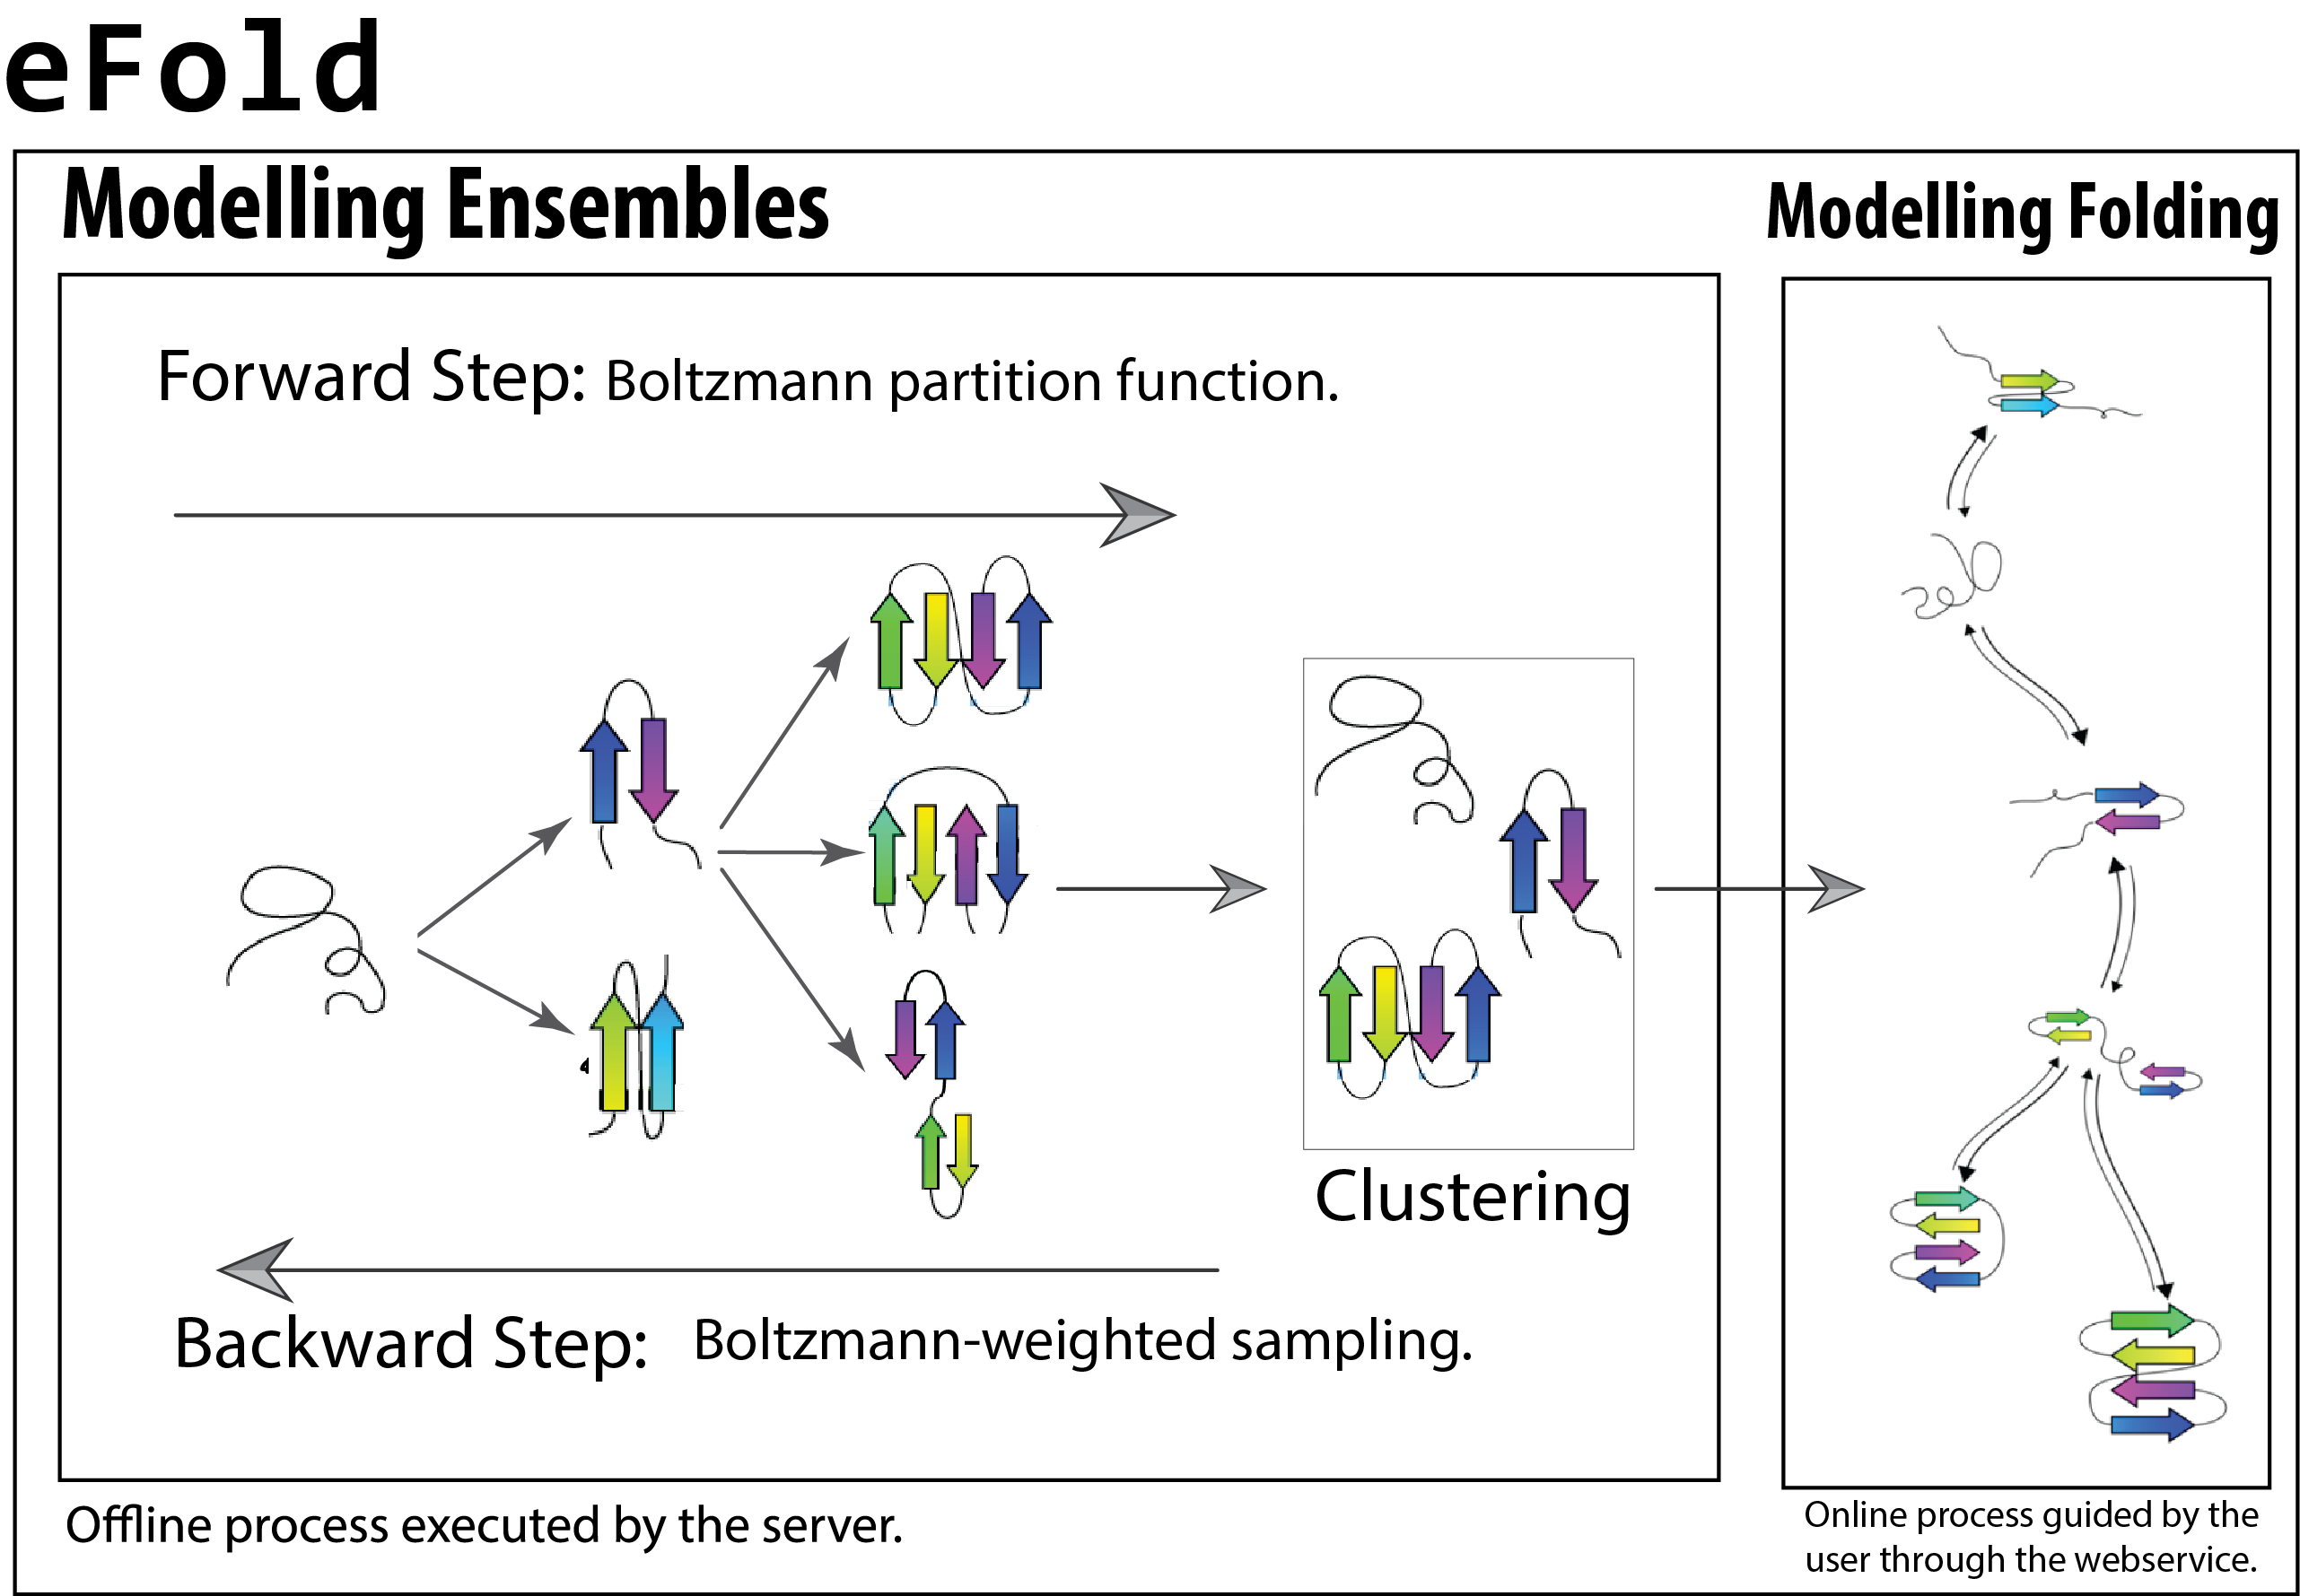
\includegraphics[scale=0.8, clip=true]{Figures/Method.png}
			\caption{\textbf{\efold:} is the proposed algorithm for predicting protein folding pathways and topologies using ensemble modelling and genomic variation. The algorithm is divided in two main phases, the modelling of ensembles and the modelling of the predicted folding dynamics. The first phase is computed off-line and it consist of a forward and backward traversal over the tree that model the hierarchical folding mechanism and that stores all the possible proteins states with its respective energies and likelihoods of occurrence. The second phase simulates the protein population dynamics based on the clusters computed in the previous phase. Specifically,  the transition from a random coil to the native state was modelled thorough a hierarchical assembly folding mechanism and it is represented as a path in a graph of varyingly folded protein conformation states. In this graph, the vertices are represented by energetically accessible conformation states presented in the clusters. The edges in the graph represent the possible folding pathways and the existence of structural similarity between the connected vertices. The user can change the structural similarity cutoff in order to generate different predicted protein pathways.}  
		\label{fig:method}
\end{figure*}

%\begin{figure*}[htbp]
%	 \centering
%	 		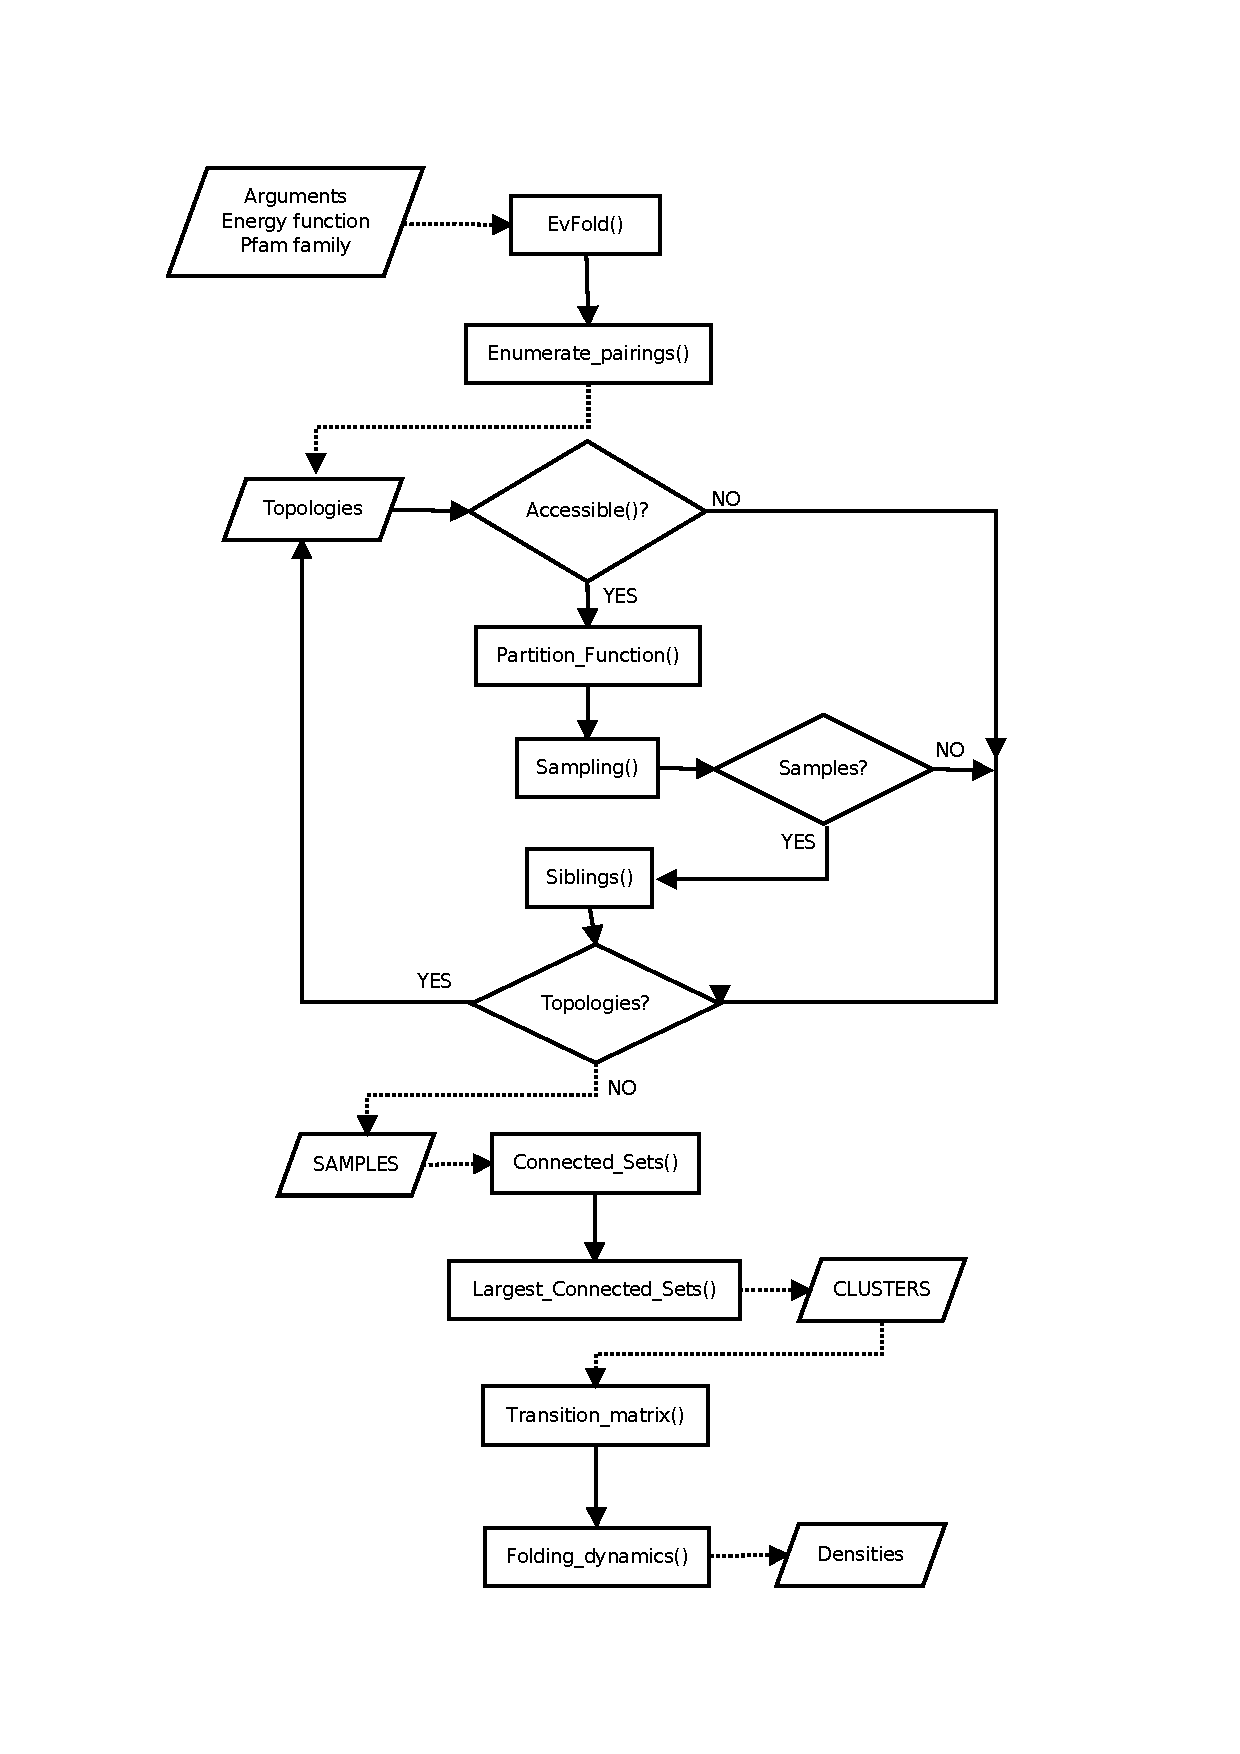
\includegraphics[scale=0.8, clip=true]{Figures/Flowchart.pdf}
%			\caption{\textbf{\efold Flowchart:} .}  
%		\label{fig:flowchart}
%\end{figure*}

\subsection{Modelling the ensembles}
\subsubsection{\textbf{The forward step.}}
The main task of the forward step in the modelling of ensembles, is to compute the partition function of secondary structures with arbitrary $\beta$-strand topologies. In order to accomplish this goal,  a statistical mechanics framework to compute the set of all possible secondary structure conformations that a protein can attain was defined. This framework is characterized by the implementation of a protein representation, the generation of all the  admissible $\beta$-sheet topologies following the proposed protein representation and the  computation of the  Boltzmann partition function over those topologies.\\


\emph{\textbf{Computation of the Partition Function:}}

Conceptually, each protein structure was described by a coarse-grained residue-level representation. Specifically, the structure was defined by the set of residue/residue contacts that form hydrogen bonds between $\beta$-strand backbones. The protein representation includes side-chain orientation and long-range contacts, that will enable us to develop an efficient strategy to enumerate all potential states. This representation sufficiently reduces the complexity of the conformational search, although, the number of protein conformations are still greatly flexible (E.g. permutation of strands, strand's size, orientation of side chains, secondary structure motifs, etc.), and the structures can take on various conformations that are vastly different between them, and the native conformation.

The protein generic topologies were encoded using a stepwise permutation algorithm through the labeled set of $\beta$-strands $\{1 \dots n\}$. For each permutation, the set of all $\beta$-strand$/$$\beta$-strand pairings were computed, such that each interaction in the $\beta$-topology is assigned to be parallel (P), anti-parallel (A) or none (N)  (See Figure \ref{fig:topologies}). It is important to stress that in order to avoid unrealistic general protein shapes, optimize computation resources and focus in valid motifs, we imposed that valid foldings must satisfy steric and biologically derived constraints. More specifically, we set a minimum and maximum strand length and minimum inter-strand loop size for the protein conformations.

Contrary to our previous implementations, the computation of all protein topologies is performed using a tree data structure, where each level of the tree contains all the topologies with a specific number of strands. Then, the first level (i.e., the root) of the tree correspond to the topologies containing the unfolded scheme, the second level of the tree contains the topologies with two strands, and so on until the leaves of the tree (i.e., $n$-level) are stored with topologies having $n$ strands. The tree is a balanced tree, for which each node (except the root) has one node parent, $m-1$ sibling nodes and $m$ children nodes. All the parent nodes share a structure with their children, where two topologies share their structures if they are identical to each other, modulo the addition or removal of a single strand pairing.

Having a tree as a data structure is important for four main reasons: $i)$ It guarantees the algorithm correctness, given that all the possible offsprings are traversed. Additionally, It ensures an exhaustive and non-overlapping count of all protein structures and it support a hierarchical assembly folding mechanism to narrow the conformation search (See the section Folding Dynamics for details) $ii)$ A Boltzmann sampling procedure can be efficiently computed using a depth-first search approach (DFS). Furthermore, the tree should not be completely filled in order to perform the procedure (see Sampling subsection). $iii)$ Pruning methods can be computed over many branches of the tree previously computed. The pruning of the three will keep the memory complexity in tractable terms, furthermore it will avoid the degradation of their performance (avoiding collisions and crossing the hash load factor). $iv)$ The tree data structure can be traversed in different fashions allowing the analysis of a highly diverse set of experiments. %See Figure ~\ref{fig:tree} for an example of the computed tree.

%In order to implement the search approaches on the tree (i.e., BFS and DFS), a recursion that guarantee the correct make up of the states in the tree is required. Then, it is desired that the offspring scheme nodes present a compatible topology with their parents, that the structural similarity can be easily computed and that all the energies of intermediate structures have been already computed by the ancestors in order to compute the recursion. In the proposed recursion, the offsprings nodes are built adding new strands to the parent topology. Particularly, new strands going from $i=2$ to $i=size of the parent$ are . The previous approach allowed us to built the tree shown in Figure ~\ref{fig:tree}. It is important to stress the following features of  the tree: i-) It is balanced tree. ii-) All the nodes belonging to the same level have the same number of children. iii-) For each node, the number of offsprings is one more than the number of offsprings of his parent. iv-) Each added strand (i.e., last column in the template) is part of a ordered sequence of numbers that goes from $i=2$ to $i=$size of the template. 


The tree structure is filled using a breadth-first approach (BFS). In other words, the level $i+1$ would not be considered until all the instances of level $i$ have been computed. The filling of the tree consists in the computation of the Boltzmann partition function $Z$ for all the nodes of the tree (i.e., all admissible $\beta$-sheet schemas). Conceptually, each structure with a specific topology is described by the set of residue/residue contacts that form hydrogen bonds between $\beta$-strand backbones. Then, we compute for each conformation a pseudo-energy which is determined by the specific residues involved in contacts. The residue/residue contact energy is computed through a potential-energy scoring function derived from frequency observations of specific residue/residue interactions in experimental data \cite{waldispuhl2006predicting}. Particularly, an energy $E_{i,j}$ is given to each residue/residue pair following Equation \ref{eq:potentials_initial}, where $Z_c$ is a statistical re-centering constant and $p(i,j)$ is the likelihood of these two residues appearing in a $\beta$-sheet environment, as observed across all nonsequence-homologous solved structures in the PDB. 
\begin{equation}
E_{i,j} = -RT[log(p(i,j)) - Z_c]
\label{eq:potentials_initial}
\end{equation}
A predicted energy is then related to the sum of potentials for all residue/residue interactions (see Equation \ref{eq:potentials}), where $i$, $j$ represent the positions of the amino-acids being computed that belongs to all the possible residue pairs $\gamma$. Further, we assign separate likelihoods based on the
hydrophobicity of the environment on either face of a $\beta$-sheet.
\begin{equation}
E(S_{n}) = \sum_{i,j \in \gamma} E_{i,j}
\label{eq:potentials}
\end{equation}
The Boltzmann partition function $Z$ can be calculated over all protein structural states to characterize the energetic landscape of a specific ensemble (see Equation \ref{eq:partition}), where $E(S_{i})$ is the free energy of the structure for the input sequence, $R$ is the gas constant and $T$ is the absolute temperature.
\begin{equation}
Z = \sum_{i =1}^{n} \exp [-E(S_i)/RT]
\label{eq:partition}
\end{equation}
With the partition function $Z$ available, the Boltzmann probability for all the structures  can then be computed using Equation \ref{eq:probability}. Therefore, the Boltzmann probability statistically characterizes the ensemble.
\begin{equation}
P(S_i) = \frac{ \exp [-E(S_i)/RT]}{Z}
\label{eq:probability}
\end{equation}

The enumeration of all possible structures is infeasible during the computation of the partition function. We have previously shown that a dynamic programming approach is an efficient method to compute arbitrary single $\beta-$sheet fold topologies. In this work, we propose a much more efficient method using a tree data structure and memoization techniques.  

\begin{equation}
E(S_{n}) = E(S_{n-1}) + Pair(s_{n-1},s_{n})
\label{eq:recursion}
\end{equation}

Equation \ref{eq:recursion} represent the recursion to compute the energy of a structure with $n$ strands, where $E(S_{n-1})$ is the interaction energy between the first $n-1$ strands, and $Pair(s_{n-1},s_{n})$ is the energy of the pairing of strand $n-1$ with strand $n$ (See Figure \ref{fig:topologies}a). The implemented recursion function exploits the shared sub-structures between schemes in the ensemble using a memoization approach. Each recursive call  compute the energy function of a specific instance and store this value in a hash table indexed by an identifier. Subsequent recursive calls, which involves the same instance, will perform a search in the tree and a table lookup instead of re-computing the value of the recursion.  

A hash table maps \textit{keys} to \textit{values}. In our implementation, \textit{keys} are lists of four indices $i_i, i_2, i_3, i_4$. These indices partition the protein structures based on the boundaries of region occupied by the strands (See Figure \ref{fig:topologies}b). The \textit{values} correspond to an array that contains information about the templates, the best computed Boltzmann partition function $Z$ and a value representing the relative abundance (likelihood) of the structure. These likelihoods are finally weighted using an evolutionary contact prediction method in order to circumvent the inherent limitation of potential energy scoring schemes.


\begin{figure}[htbp]
			\centering
	 		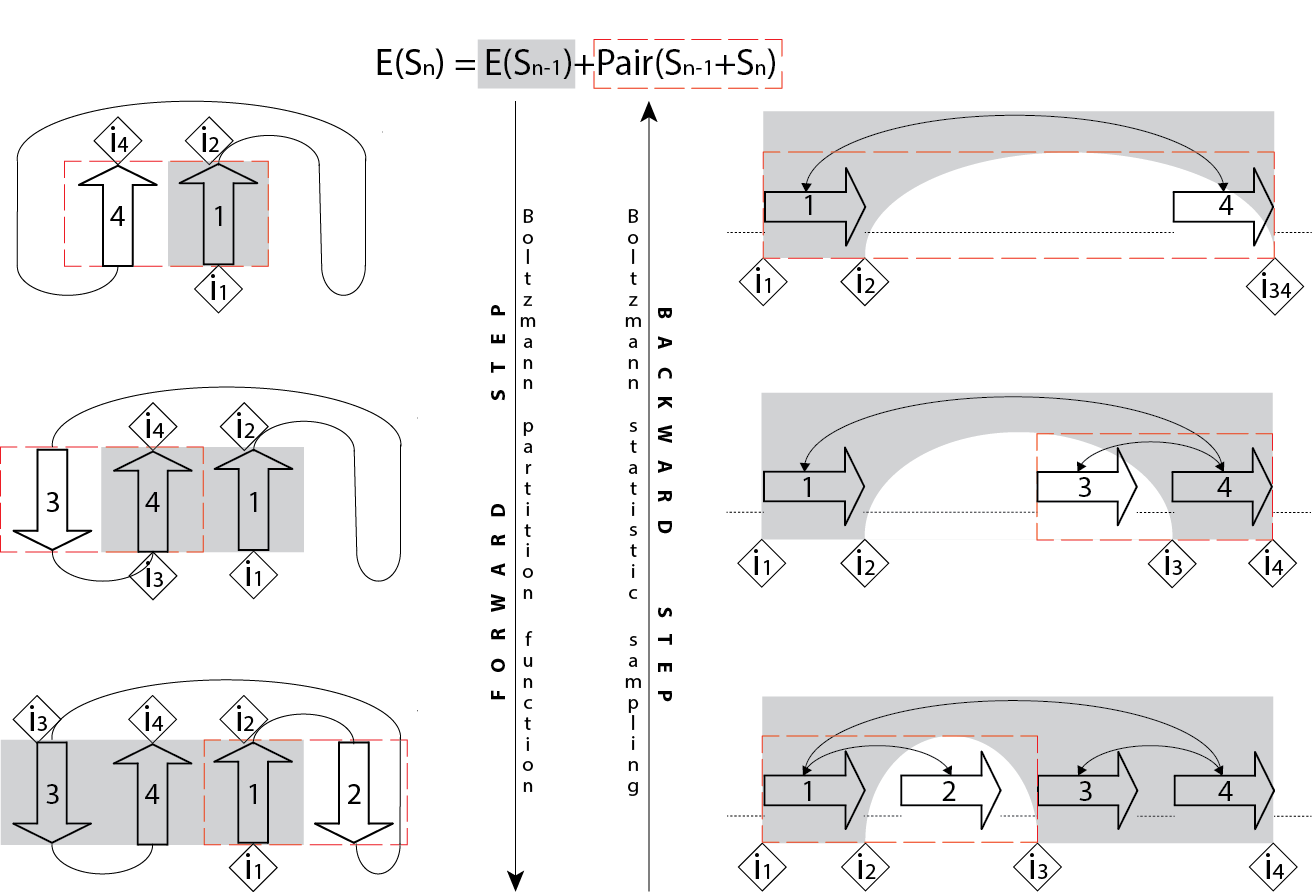
\includegraphics[scale=1.35, clip=true]{Figures/Topologies.png}
			\caption{\textbf{\efold Topologies:} \textit{3A4P1A2} is the protein topology for the proteinG}  
		\label{fig:topologies}
\end{figure}



%\begin{figure*}[htbp]
%	 \centering
%	 		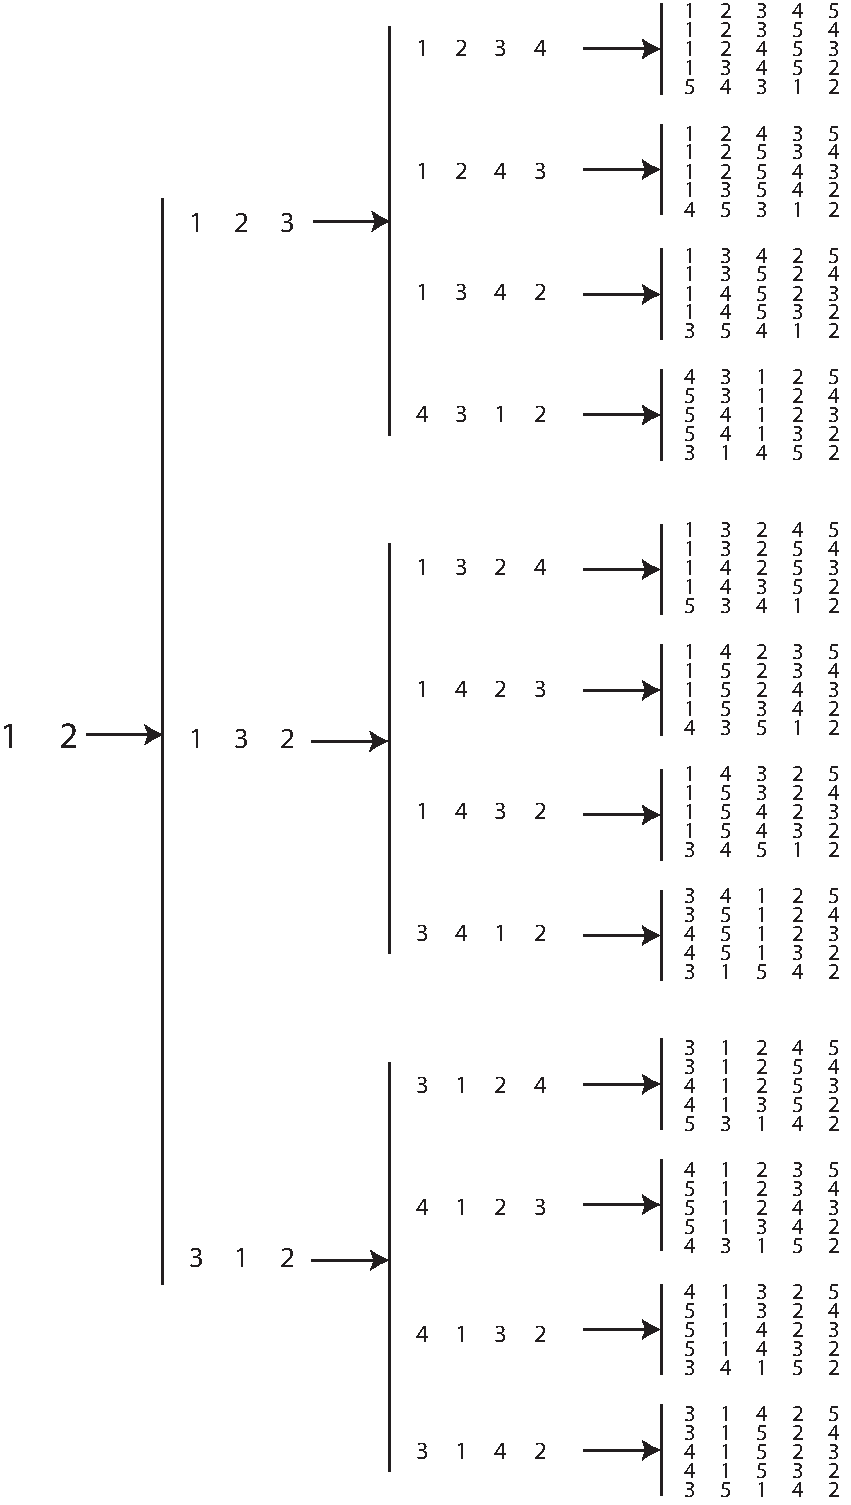
\includegraphics[scale=1, clip=true]{Figures/Tree.pdf}
%			\caption{}  
%		\label{fig:tree}
%\end{figure*}

%\emph{\textbf{EvFold()}} 
The used evolutionary contact prediction method \cite{marks2011protein}, called \evfold, is based on a maximum entropy approach to perform an unsupervised inference of residue-residue contacts from multiple sequence alignments (MSAs). Specifically, the method derives a set of essential residue pair couplings through a maximum entropy approach and a direct coupling analysis. The minimal set of pairs predicted to co-vary due to evolutionary constraints is returned as output of the algorithm and it is connected as an heuristic to our ensemble approach. 

In our ensemble pipeline, the set of predicted couplings are ranked by their numerical values and they are codified in an $N\times N$ binary matrix $C$, also know as a predicted contact map, whose element $C(i,j) = 1$ if the predicted direct information of residues $i$ and $j$ is greater than a threshold value $t$. In our approach, $t$ was chosen as the direct information of the $500$ hundred best ranked prediction. This parameter was determined as a good threshold to predict 3D structures with correct spatial arrangement of $\alpha$ helices and $\beta$-strands for our benchmark proteins, as compared to their experimentally determined structures.

The predicted contact map $C$ is used to numerically compute residue pairs involved in secondary structure motifs. Particularly, those motifs can be recognized in the matrix $C$ identifying a cluster of contacts using geometric knowledge of $\alpha$-helices and $\beta$-strands. Then, we can add $\alpha$-helices template information to our permutable $\beta$-template procedure to enable the modelling of  pure $\beta$, pure $\alpha$ and $\alpha$/$\beta$ interactions. Now, the different sampled structures can be penalized or rewarded depending on the modelled motif. The last procedure builds a selective constraint which can intensify the signal of $\beta$-strand interactions during the modelling of pathway kinetic.

%The implemented recursion function exploits the shared sub-structures between schemes in the ensemble using a memoization approach. Each recursive call  compute the energy function of a specific instance and store this value in a hash table indexed by an identifier. Subsequent recursive calls, which involves the same instance, will perform a table lookup instead of re-computing the value of the recursion.  The values stored in each node correspond to an array that contains the information of the templates, the structure of the parent and the computed energy value. The values represent the necessary information to traceback an specific protein instance.

%Each node in the tree is labeled as a permutation of a set of $\beta$-strands (i.e., Template), however, each node also stores the values for all the pairings involving the template of the node. In other words, each node stores all the energy values for the schemas of the permutable $\beta$-sheets that consider the labeled template. Each node also stores the information (substructure energies) to compute each of the offsprings generated by the template.  Given that the added strand in each offsprings is part of a ordered sequence of numbers (going from $i=2$ to $i=size of the template$), each specific node has to store the information needed as substructures for the next level. Particularly, all the configurations that will allow the addition of a new strand $i$, for $i=2\dots i= $goes from $i=2$ to $i=size of the template$, must be independently stored. Figure ~\ref{fig:tree_details} shows how the computation of the Z score is performed for the template $1 2 3 4 5$. Specifically, it only needs the substructures stored (which have been already computed) in the parent node and that are known to have enough space in the sequence to add a new strand in the position $5$ (see the red circle area in template $1 2 3 4$). The underlined red circle areas in the other tree leves are drawn as a reference of the path followed by the substructures to compute the template $1 2 3 4 5$, however, it must be clear that no re-computation or look up table is performed over those tables.    

%\begin{figure*}[htbp]
%	 \centering
%	 		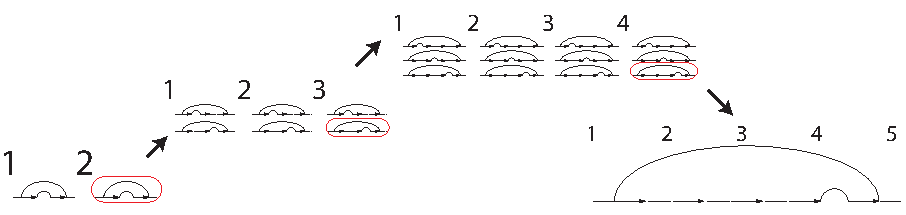
\includegraphics[scale=1.2, clip=true]{Figures/Tree_details.pdf}
%			\caption{}  
%		\label{fig:tree_details}
%\end{figure*}

%The proposed data structure presents the following improvements with respect to our previous implementations.
%\begin{itemize}
%\item \tfolder re-computed all the permutable $\beta$-schemas of a set of instances with shared structures (Two instances share their structures if they are identical to each other, modulo the addition or removal of a single strand pairing). With the new implementation, this re-computation is avoided through a table lookup from the node of the parent node.
%\item \tfolder fails to compute the complete set of $\beta$-schemas once a threshold of $5$ strands has been gotten. With the new implementations, the computation of all $\beta$-schemas until a threshold of $6$ strands is guarantee.
%\item \tfolder computes the protein topologies following a specific order. Particularly, it builds the topologies adding strands from left to right. For example, in order to compute the template $1~2~3~4~5$, \tfolder will create the templates $1 ~ 2$, then, it will add the left most strand (i.e., strand $3$) to create the template $1~2~3$. \tfolder will go on with this process (adding in order the templates $4$ and $5$) until the final template is achieved. On the other hand, \efold will create the topologies based on the most energy favourable templates (and not in a hard-coded order). Then, in order to create the template  $1~2~3~4~5$, \efold can start the process choosing the most favourable template for the following topologies $1~2$ or $2~3$ or $3~4$ or $4~5$.  Next, and depending on its selection, \efold is able to add strands to the left or right of the previous structure.
%\item The computation of compatible topologies is simplified and it is derived from pruning procedures over the tree.  
%\item The sampling procedure is performed as a lookup table procedure in the tree. 
%\end{itemize}








\subsubsection{\textbf{The backward step.}}

A characterization of the full ensemble of protein structures using the complete enumeration of secondaries structures is restrictive. Then, during the backward step, we compute a statistically representative sample of secondary structures. Additionally, clusters of these secondary structures are built based on their topological and structural similarities to work with a tractably sized system. This system is used as input for the prediction of folding dynamics.

During the sampling process, a statistical sampling over the protein conformations generated in the forward step is performed. Particularly, a recursive statistical algorithm to sample from the Boltzmann ensembles of secondary structures using the tables constructed to compute the partition function is used. We take advantage of the tree structure and the memoization tables to randomly draw secondary structures according to the probabilities given by equation \ref{eq:probability}. 

Since the final structure of the protein is not known, the proposed approach samples configurations from all possible $\beta-$sheet topologies (i.e., all the nodes of the tree). Then, for each node, the sampling algorithm performs a recursive traceback through the partition function tables of its parents. For a specific node, the location of a single strand is sampled from the region indicated by the indices $i_2, i_3$ (See figure \ref{fig:topologies} for an example).  

\subsection{Predicting Folding Dynamics}

In order to simulate population dynamics, we use ensemble predictions and a hierarchical assembly folding mechanism to narrow the conformation search. In this process, the secondary structure is formed according to the primary structure of the protein. Specifically, the first step in the process is represented by the unfolded state, next the secondary structures are formed and they fluctuate around their equilibrium positions. Finally, the secondary structures interact between them and they create a folding pattern that will find the native conformation. The proposed approach try to separate conformational transitions that are critical to folding from those that could simply result from minor structural fluctuations.  

Our approach predicts coarse folding transitions as described in previous models \cite{wolfinger2004efficient}. Specifically, the transition from a random coil to the native state was modelled as a path in a graph of varyingly folded protein conformation states. In this graph, the vertices are represented by energetically accessible conformation states which have been previously generated by the proposed Boltzmann ensemble sampling method (See subsection Sampling Process). The edges in the graph represent the possible folding pathways and the existence of structural similarity between the connected vertices. Specifically, for every pair of states we add an transition edge if (1) the states have compatible topologies, and further, (2) the states show structural similarity. Two states are compatible if they are identical to each other, modulo the addition or removal of a single strand pairing. On the other hand, the structural similarity between two samples is estimated through a contact based metric, where two structures are structurally similar if the contact-based metric is below a transition threshold.

Given that two states are connected in the graph, the rate at which they interconvert is proportional to the difference between free energies of the states ($\Delta G$). Since we sample thousands of states from each strand topology and  in order to work with a tractably sized system, we partition the state space into macro states using clustering. We cluster protein configurations according to contact distance metrics, and associate each cluster with a intermediate folding state. Under this approximation, we consider two clusters to be connected if the minimum distance between any two states from each is less than a threshold value. We define the ensemble free energy difference $\Delta G_{ij}$ between two macro states $i$ and $j$ by summing
over the states from which they are composed (See Equation \ref{eq:difference}). 

\begin{equation}
\Delta G_{ij}  = E(\chi_i)-E(\chi_j) = \sum_{x \in \chi_i} E(x) - \sum_{x \in \chi_j} E(x)
 \label{eq:difference}  
\end{equation}

Given the previous graph, the transition rates $r_{ij}$ between states $i$ and $j$ is calculated using the Kawasaki rule (with parameter $t_0$ to scale the time dimension (See Equation \ref{eq:transition})). Then, the change in the probability of the system being in state $i$ at time $t$ can be calculated from the total flux into and out of state $i$ (see Equation \ref{eq:flux}, where $p_i$ is the probability of state $i$, $X$ is the state space). 

\begin{equation}
 r_{ij}  = r_0 \exp(-\Delta G_{ij}/2RT)
 \label{eq:transition}  
\end{equation}

\begin{equation}
 \frac{dp_i}{dt}  = \sum_{j \in X} r_{ij}p_{j}(t)
 \label{eq:flux}  
\end{equation}

Finally, the dynamics of the system are calculated by treating the folding process as a continuous time discrete state
Markov process. Given the matrix of folding rates $R$, where $R_{ij} = r_{ij}$ and initial state density $p(0)$, the distribution overs states $p(t)$ of the system at time $t$ is given by the explicit solution to the system reported by Equation \ref{eq:ode}. Then, the distribution of conformations over folding time is estimated by solving this system.

\begin{equation}
 p(t)  = \exp (Rt) p(0)
 \label{eq:ode}  
\end{equation}


\section{Experimental Framework}

In this section, an experimental framework to report the results obtained using the proposed approach is presented. Specifically, an analysis of the results obtained over the set of benchmark proteins is provided.

In order to understand the performance of the proposed method, two main experiments were performed to study the modelling ensemble (protein structure prediction) and modelling folding phases (protein pathway prediction). The first phase is performed off line and it contributes most of the complexity of the algorithm. The second part is computed online and it runs using a web-service as interface with the user. \efold is run having as input only the amino-acid sequence and a set of parameters. Then, the algorithm runs until all the folding pathways and structures have been computed. Based on the experimental framework and user experiences with our previous techniques, we have fixed the limits of our algorithm (constrained in the web service interface) to predict the folding pathways for small proteins (less than 200 amino acids), and to model proteins with up to 7 different $\beta$-sheet strands.

\begin{table}[htbp]
\footnotesize
\begin{center} {
\begin{tabular}{c c cc cc cc}

Measure & Approach & \multicolumn{2}{c}{$x >0$} & \multicolumn{2}{c}{$x\geq12$} &
\multicolumn{2}{c}{$x\geq 24$} \\
& $$  & \multicolumn{1}{c}{$\pm 0$} & \multicolumn{1}{c}{$\pm 2$} &
\multicolumn{1}{c}{$\pm 0$} & \multicolumn{1}{c}{$\pm 2$} & \multicolumn{1}{c}{$\pm 0$} &
\multicolumn{1}{c}{$\pm 2$}\\ \midrule
\multirow{2}{*}{Precision} &   Ours  &\bf20.75 & \bf71.76  &   \bf17.65 & \bf75  &   \bf33.33 & \bf94.12\\
&   tFolder  &13.3 & 52.1  &   10.6 & 54.1  &   14.0 & 58.3\\
\multirow{2}{*}{Recall}  &  Ours   &\bf100 & \bf100  &   \bf100 & \bf100  &  25 & \bf100 \\
&   tFolder  & 56.3 & 97.9  &   53.8 & 61.5  &  \bf37.5 & 87.5 \\
\multirow{2}{*}{F-measure} &  Ours   &20.75 & \bf68  &   \bf35.48 & \bf87.1  &  \bf61.11 & \bf100 \\
&    tFolder & \bf21.5 & \bf68  &   18.1 & 69.2  &  20.3 & 70 \\

\end{tabular} }
\end{center}
\caption{\footnotesize The performance of the proposed approach for contact prediction is evaluated based on the precision, recall and F-measure of experimentally observed contacts. The performance metrics are reported for contacts which are 0, 12 and 24 residues apart. The metrics are also studied when predicted contacts are within $\pm 2$ residues of an observed contact. The best results obtained are shown in bold.}
\label{tb:comparison}
\end{table}

\subsection{Contact and Strand Prediction}

The prediction of residue-residue contacts has been proved useful in reconstructing protein backbones by providing information to determine accurate 3D protein structures. Generally, the predictors of residue-residue proximity in folded structures (such as \evfold) are based on the existence of interdependent changes in groups of variable amino acids belonging to a protein family of homologues. Even if \efold is not an algorithm developed to predict residue-residue contacts, we evaluated the prediction capabilities of \efold to recognize contacts involved in secondary structures. Then, we tested the proposed algorithm using the complete protein benchmark and compared the performance of \efold with the predictions performed by \evfold and by our previous algorithm \tfolder. 

The first experiment quantify the ability of \efold to predict protein topologies through the prediction of  residue-residue contacts. We sample 150 configurations for each protein of the benchmark, and use these ensembles to compute a stochastic contact map. The contact map represents the probability of observing a given contact. Contacts are defined as all $C_\alpha$ atoms less than $8\AA$ apart in the PDB file. The precision (i.e., $\frac{no. ~ of ~ correctly ~ predicted ~ contacts}{no. ~ of ~ predicted ~ contacts}$), sensitivity (i.e., $\frac{no. ~ of ~ correctly ~ predicted ~ contacts}{no. ~ of ~ observed ~ contacts}$) and F-measure {i.e., $\frac{2 \times precision \times sensitivity}{precision + sensitivity}$} were the chosen measures to assess the effectiveness of the method. These metrics are evaluated for all types of contacts (short, medium, and long-range). Particularly, an evaluation is performed when predicted contacts are within exact or $\pm2$ residues of an observed contact, and are more than 0, 12 and 24 residues apart. 

Figure \ref{fig:boxplots} (column \textit{Contact prediction}) reports, through box plots, the best results of the experiments for the complete set of proteins (row \textit{Complete}) and the set divided by the number of strands in the tested proteins. It is important to notice that the proposed method predicts residue contacts with an excellent precision for $\pm2$ for all contact separations in the complete benchmark. The precision for exact prediction (i.e., columns $\pm0$) is also high and it averages around $50\%$ for the short and medium contacts and around $33\%$ for long-range contacts. This result is significant given that critical protein folding steps can involve both short range and long-range $\beta$-sheet contacts and that the precision assessed state-of-the-art algorithms in contact prediction for proteins without homology-based templates averages around 20\% \cite{monastyrskyy2014evaluation}. The recall obtained by \efold average around $10\%$ and $30\%$ for contacts $\pm 0$ and $\pm 2$, respectively. This results is low as expected given that \efold does not aim the prediction of all residue contacts, but those involved in secondary structures. 

Comparing the predicted residue contacts between \efold and our previous model \tfolder for the Protein G, it is worth noticed in Table \ref{tb:comparison} that \efold shows a better predicted accuracy than the \tfolder algorithm. Furthermore, the proposed method performed better than tFolder in all the ranges except for the exact observed contacts studied 24 residues apart. The proposed approach not only kept sensitive to the distance of contact separation, but it increased the precision and sensitivity of the ensemble method. 

\efold is also compared with \evfold to measure at which extent \efold improve the residue contact predictions used as input in our method. Particularly, the $500$ best ranked evolutionary inferred contacts (i.e., EICs) computed by \evfold are used as input in \efold (see section Methodology for more details).  Figure \ref{fig:boxplotsevfold} (column \textit{Contact prediction}) reports, through box plots, the results of the experiments for the complete set of proteins. The recall of \evfold for $\pm2$ averages around $40\%$ for all the range of contacts. Then, \evfold gets a better coverage than \efold given that, unlike \efold, \evfold does not focus only in contacts involved in secondary structures. Regarding the precision of the \evfold results, its low performance can be explained by the dependence of \evfold on the depth of the target alignments (See supplementary Table 1 for a complete list of the size of MSAs).  Figure \ref{fig:boxplotsevfold} shows that the methodology implemented by \efold improved the initial contact predictions performed by \evfold. 

As previously stated, \efold is an ensemble algorithm aimed at protein structure and pathways prediction. Then, we are interested in study its capability to predict contacts involved in secondary structures. The prediction of those contacts is studied following the same methodology than normal residue-residue contacts. A pair of residues are considered to be part of $\beta$-strand interactions if the predicted residues are contacts and those contacts are observed to be involved in a $\beta$-sheet interaction in its corresponding PDB file. Finally, the topology prediction is studied based on the ranking of the Boltzmann probabilities of each ensemble of secondary structures. Particularly, the position of the topology reported by the PDB file with respect a sorting of the Boltzmann probabilities of all the secondary structures is computed.  

Figure \ref{fig:boxplots} (column \textit{Strand prediction}) reports, through box plots, the best results of the experiments for contact prediction of residue-residue contacts involved in $\beta$-sheet structures. The results are spliced in rows showing the complete set of proteins (row \textit{Complete}) and the set divided by the number of strands in the tested proteins. It is important to notice that the F-measure values for $\pm2$ for all contact separations in the complete benchmark is higher than $60\%$. This result correspond to a very good performance of the method in terms of its accuracy and sensitivity. Furthermore, it confirms \efold as a very good predictor of contacts involved in secondary structures. Regarding the exact prediction (i.e., columns  $\pm0$), the precision decreases for long range contacts. Particularly, it  goes from a precision around $30\%$ for the complete set of contacts to a precision around $20\%$ in long range contacts. The best and worst performance of \efold can be recognized in proteins with three and two strands, respectively. It is important to stress that in \efold there is not a big difference between the precision and sensitivity values for strand predictions, given that \efold focuses on predicting contacts involved only in secondary structures.

Figure \ref{fig:boxplotsevfold} (column \textit{Strand prediction}) reports, through box plots, the results of the experiments performed by \evfold for the complete set of proteins. It is important to notice that these results are more homogeneous than the results obtained in the contact prediction experiment. Moreover, there is not a big difference in the behaviour of the precision and recall measures, as noted in the contact prediction column. There is not a big difference either between the contacts $\pm 0$ and $\pm 2$ for all the contact ranges. The average of all the evaluation measures for an exact prediction ($\pm 0$), for the strand prediction experiment, fall in the same range (i.e., below a $10\%$) than its contact prediction counterpart.  Then, it gives the insight that most of the contacts predicted by \evfold are involved in secondary structures. On the other hand, there is a clear decrease of the recall of the strand prediction with respect to the contact prediction, suggesting that for ($\pm 2$) predictions, \evfold reports a greater quantity of contacts not involved in secondary structure than the exact predictions ($\pm 0$).  The prediction values for \evfold are much lower than the values of \efold, showing that the methodology implemented by \efold improved the initial contact predictions performed by \evfold regarding contact and strand predictions. 

There is not a clear consensus about what accuracy, coverage, and distribution of contacts along the sequence are needed to 
improve the prediction of protein structures and/or pathways, however, in general the incorporation of contact information into protein folding programs leads to improvement of the results. Particularly, the correct prediction of long-range contacts must be predicted correctly to allow an accurate folding pathways to be reconstructed. Long-range contacts narrows the search space of possible conformation imposing strong constraints on the 3D structure. \efold represents an ensemble predictor that is conceptually different to the state-of-the-art algorithms in contact prediction, however, it produce results comparable results with those algorithms. Furthermore, \efold reports very good results, when compared with standard evaluation measures, for contact and residue prediction.  




\begin{figure*}[htbp]
	 \centering
	 		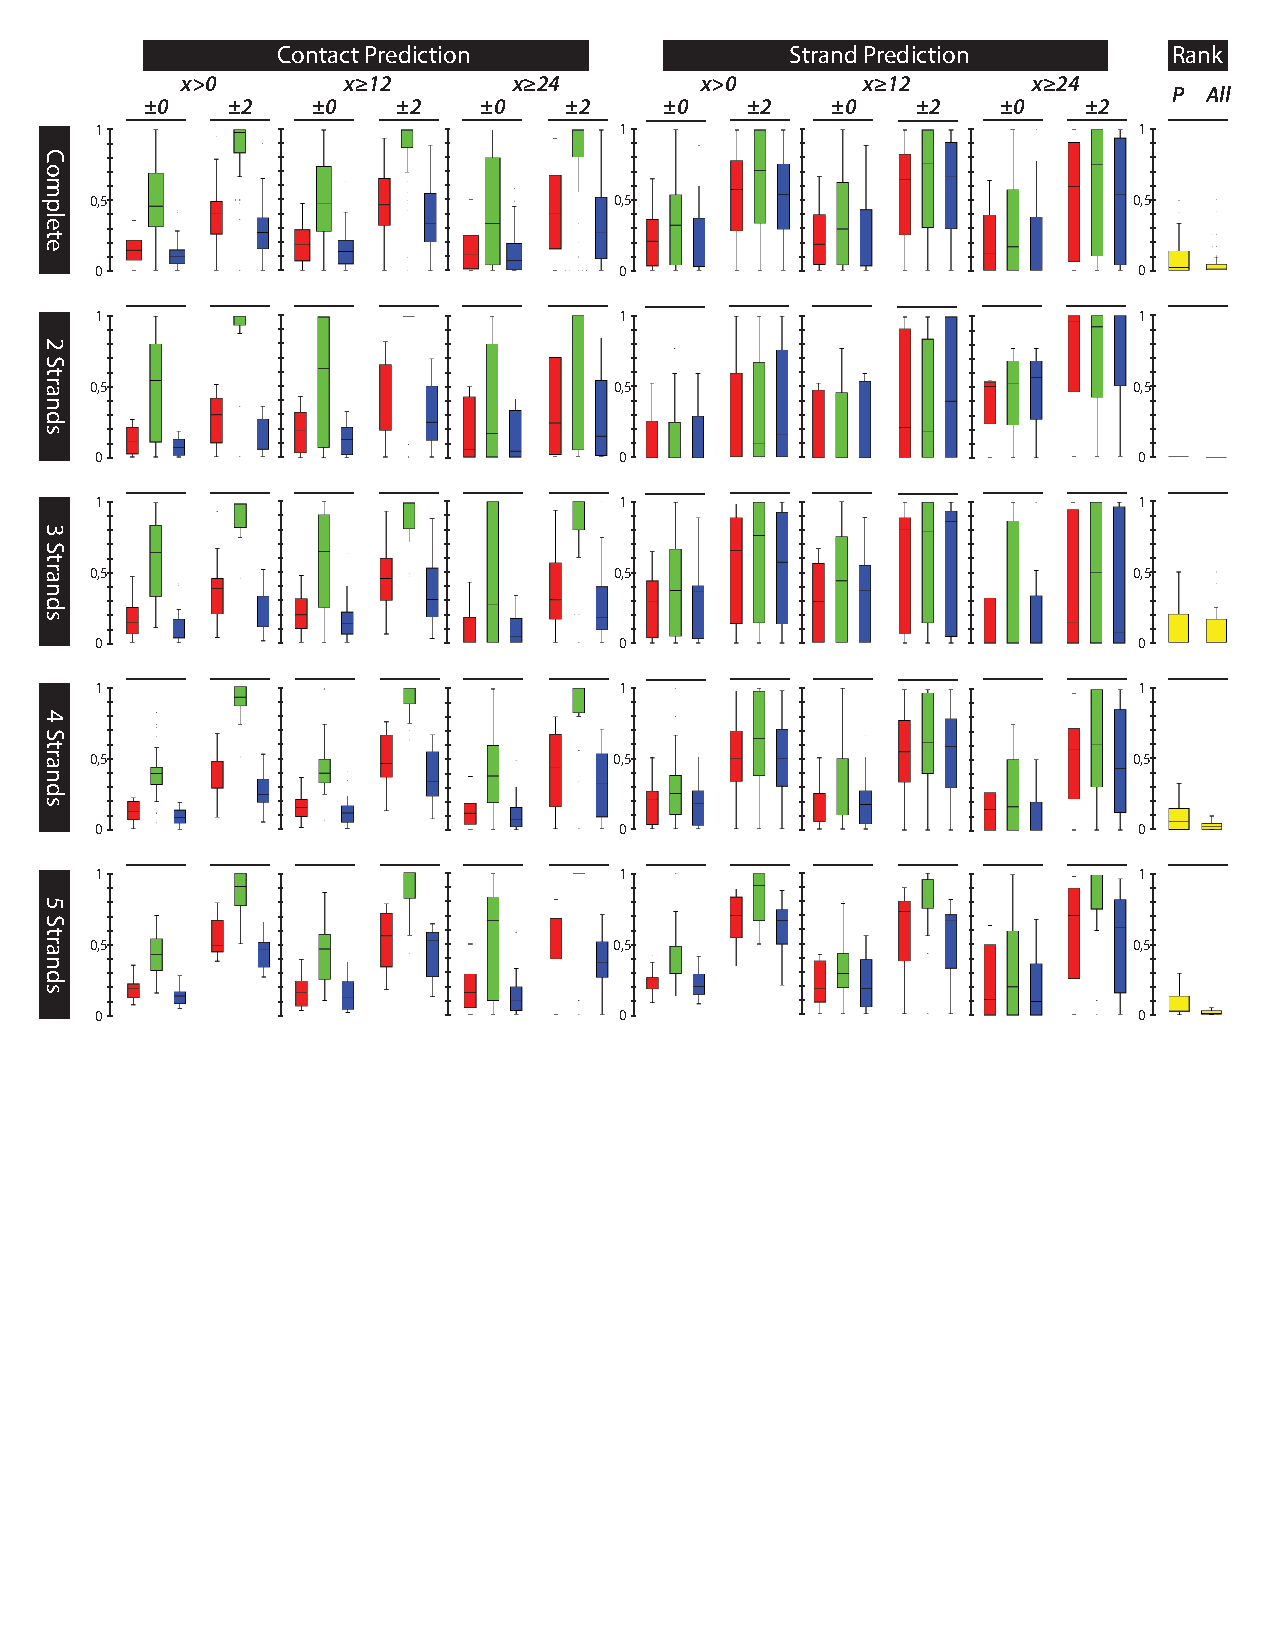
\includegraphics[scale=0.85, angle =0, clip=true, trim= 20 285 0 2]{Figures/BoxPlots.pdf}
			\caption{ The performance of the proposed approach for contact prediction is evaluated based on the precision(green), recall(blue) and F-measure(red) of experimentally observed contacts. The performance metrics are reported for contacts which are 0, 12 and 24 residues apart. The metrics are also studied when predicted contacts are within $\pm 2$ residues of an observed contact.}  
		\label{fig:boxplots}
\end{figure*}

\begin{figure*}[htbp]
	 \centering
	 		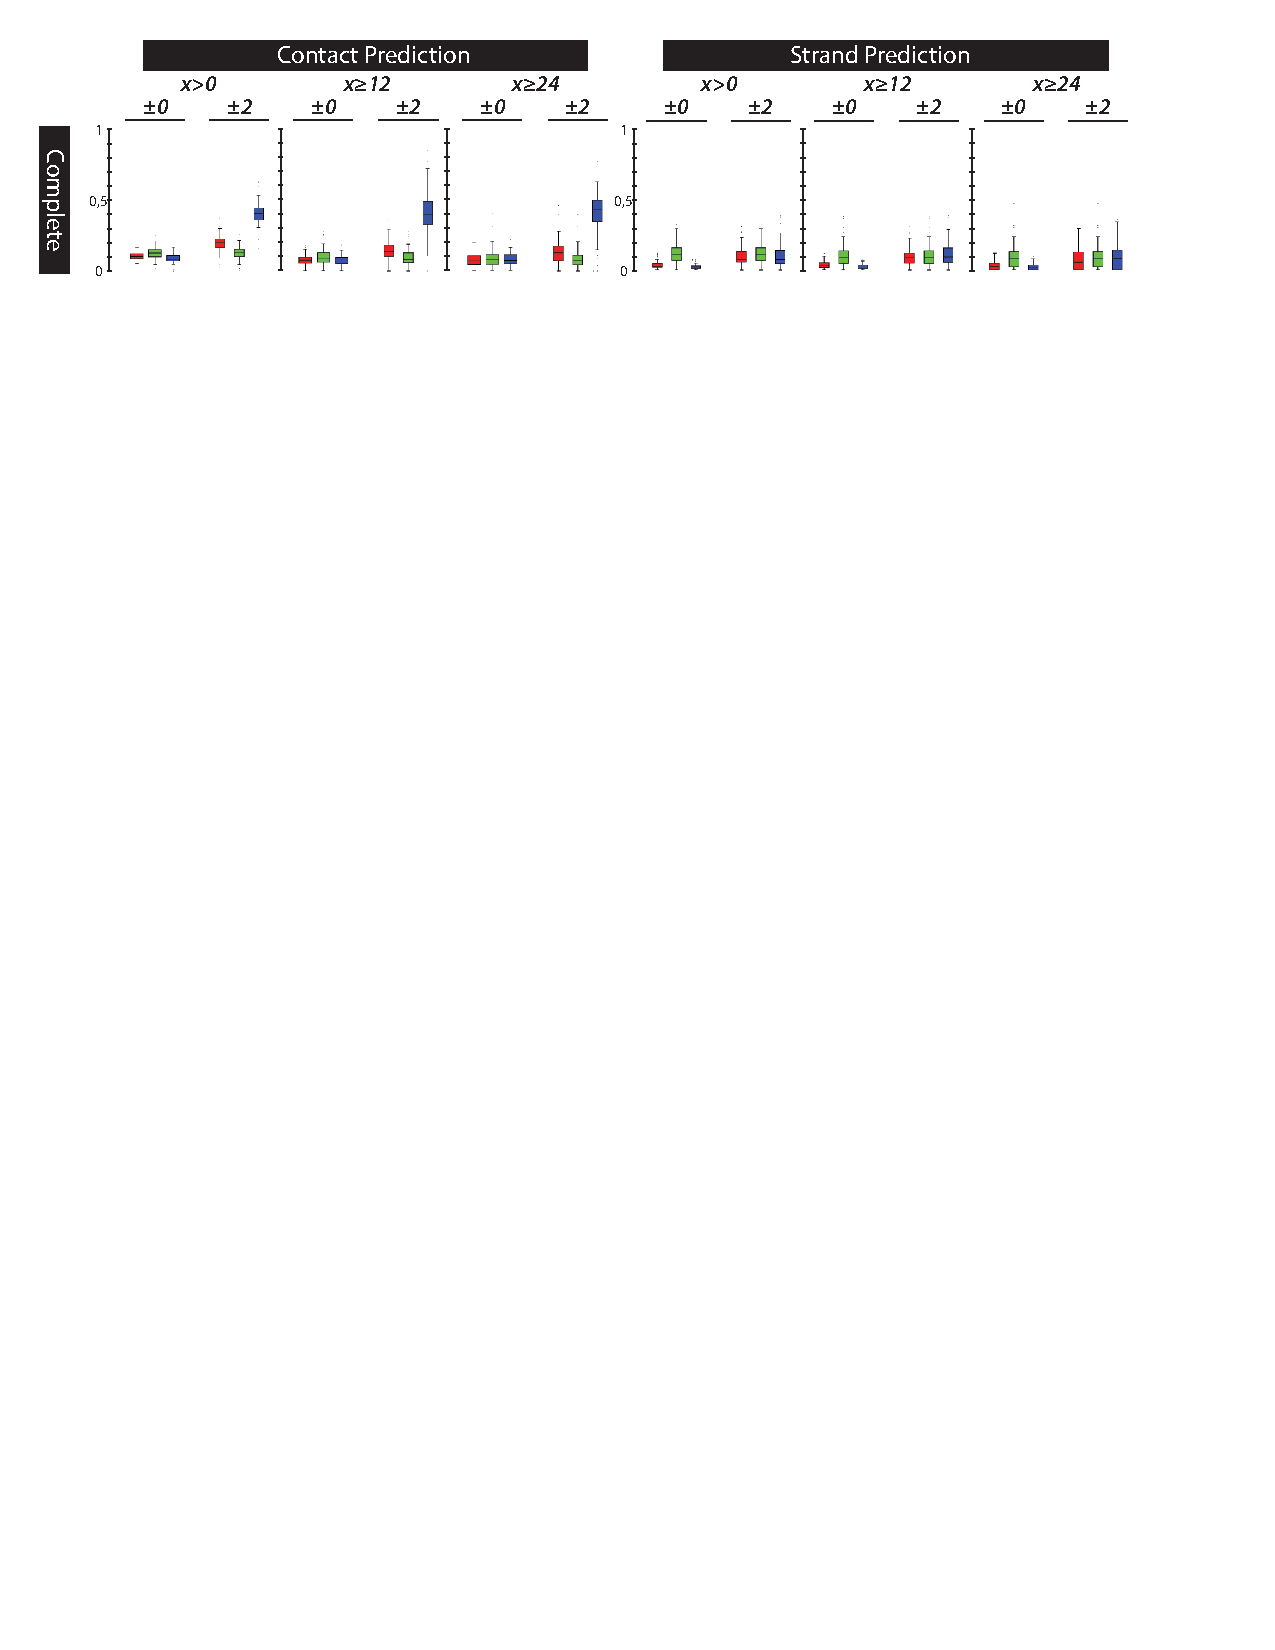
\includegraphics[scale=0.9, angle =0, clip=true, trim= 20 650 50 20]{Figures/BoxPlotsEvFold.pdf}
			\caption{ The performance of \evfold for contact prediction is evaluated based on the precision(green), recall(blue) and F-measure(red) of experimentally observed contacts. The performance metrics are reported for contacts which are 0, 12 and 24 residues apart. The metrics are also studied when predicted contacts are within $\pm 2$ residues of an observed contact.}  
		\label{fig:boxplotsevfold}
\end{figure*}


\subsection{Protein Topologies Prediction}

\efold represents the proteins by a coarse-grained residue-level representation using the set of residue/residue contacts that form hydrogen bonds between $\beta$-strand backbones. \efold performs the generation of all the admissible $\beta$-sheet topologies and the computation of the Boltzmann partition function over those topologies. Then, \efold ranks those topologies based on their energy states and it clusters the top low-energy states to predict the folding dynamics. The experiment reported in this section quantify the ability of \efold to correctly rank the admissible $\beta$-sheet topologies. Particularly, for each protein in the benchmark, we are interested in quantify the position of the topology reported by the corresponding PDB file in the rank computed by \efold.

Figure \ref{fig:boxplots} (column \textit{Rank}) reports, through box plots, the position occupied by the PDB topologies in the ranking computed by \efold. Particularly, for each protein composed by $L$ strands, the position with respect to the top percentage when considering all the topologies with $L$ strands (column \textit{All}) and the attainable topologies given a common parent with $L-1$ strands (column \textit{P}) are computed. It is important to stress that the likelihood of a specific topology to be chosen by \efold to create clusters of low-energy states (used to predict the folding dynamics) increases as the topology move to the head of the ranking-list.

Figure \ref{fig:boxplots} (column \textit{Rank}) shows that, in average, the proposed approach ranks the target topologies (i.e., the topologies reported in the PDB) in the top $2\%$ for the categories \textit{All} and \textit{P}. The best performance is computed for proteins of two and five strands. On the other hand, the worst performance is computed by proteins of three strands. \efold performs better when the ranking is computed for all the the admissible $\beta$-sheet topologies (column \textit{All}), than when compared with a subset (column \textit{P}). Figure \ref{fig:boxplots} (column \textit{Rank}) shows excellent discrimination power of \efold to separate conformational transitions that are critical to folding from those transitions that could simply result from minor structural fluctuations. In other words, \efold allows the sampling of accurate conformations and it also score accurately those models more favourably from other decoys.   


\subsection{Protein Pathway Prediction}

To study the efficacy of our technique for predicting protein folding pathways, we studied the folding landscape of proteins for which their pathways have been elucidated through many experimental studies and/or MD simulations (see Material section for more details). A graph for a specific folding pathway was constructed by considering all pairs of clusters computed  during the modelling ensemble phase. If the minimum distance between two clusters was less than the transition threshold, we considered that there was exchange between the two states. 

\subsubsection{Protein G}







 The edges in the graph represent the possible folding pathways and the existence of structural similarity between the connected vertices. Specifically, for every pair of states we add an transition edge if (1) the states have compatible topologies, and further, (2) the states show structural similarity.


shows how the probability of observing any of the reachable states changes over time. Inspection of this figure reveals that the folding intermediates are consisted with previous literature reports. Specifically, it is consistent with the work reported by (\cite{blanco1994short,kuszewski2008fast}), with respect to the early formation of the second hairpin ($\beta3 - ~turn -\beta4$) and its fundamental role in the folding process. Additionally, this second hairpin centers around known nucleation points W43, Y50, F54 that are strongly stabilized by three hydrophobic residues W43, Y45 , F52 (\cite{hubner2004commitment}). Our results also show the nucleation of the $\beta$-sheet residues between $\beta1$ and $\beta4$ as a next folding event (See permutation $3 ~ 4 ~1 ~2$ with pairings  $\mathit{ANTI ~NONE ~ANTI}$). This folding event can be preceded by the folding interaction between the $\alpha$-helix and the second hairpin as also reported in (\cite{kmiecik2008folding,song2002path}). 


Comparing the predicted folding pathways between \efold and our previous model \tfolder (See Supplementary Figure TBD), it is worth noticed that both models were able to predict the reported pathway for the tested protein; however, the probability of the experimental folding pathway is higher for \efold than \tfolder. The previous fact means that \efold was more likely to correctly predict the observed folding pathway than its counterpart. Additionally, it is clear that \efold was able to narrow the number of generated and predicted templates. There are two main factors that could help \efold to got this performance with respect to \tfolder. $i)$ The penalization term used in \efold, which penalizes the protein conformations that superimpose a $\beta-strand$ where an $\alpha-helix$ structure was predicted, allowed the model to narrow the search around conformational transitions that are critical to folding. $ii)$ The hierarchical assembly folding model used in \efold could represent a step-wise mechanism to narrow the conformation search through the correct prediction of the  the initial stages of protein folding process.







\begin{figure*}[htbp]
	 \centering
	 		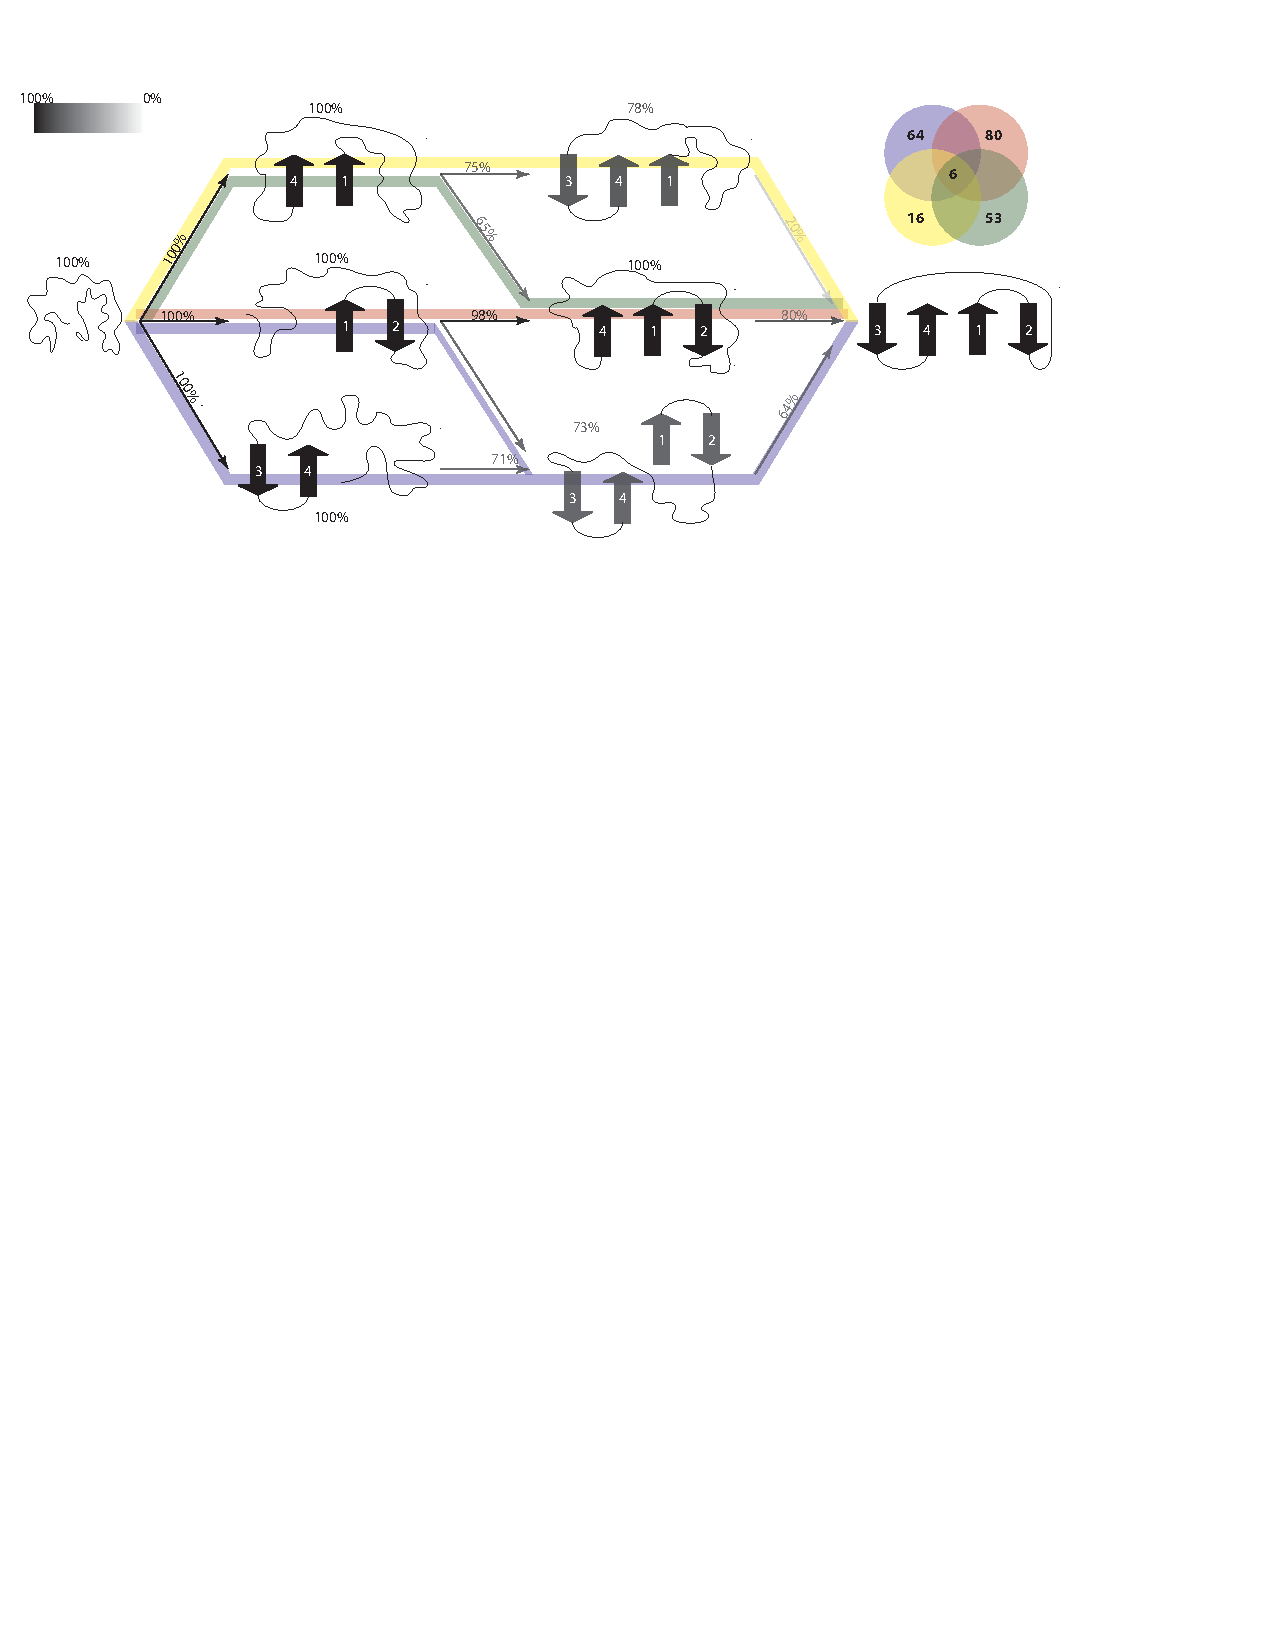
\includegraphics[scale=0.9, angle =0, clip=true, trim= 10 525 100 40]{Figures/Pathways_1EM7.pdf}
			\caption{Pathways 1EM7: Figure \ref{fig:Pathways_1EM7} represents the predicted transitions from a random coil to the native state of proteinG as a path in a graph of varyingly folded protein conformation states. The states in the graph represent energetically accessible conformation states which have been previously generated by the proposed Boltzmann-weighted ensemble sampling method. The percentage at top of each vertex (and its corresponding transparency) count for the number of times that this topology is predicted as a transition over the total number of runs. The vertices in the graph represent the transition between two topologies. The topologies connected by an edge are compatible topologies with structural similarity. The percentage at top of each edge (and its corresponding transparency) count for the number of times that this transition is found over the total number of runs. The predicted folding pathways are presented as paths in the graph. The percentage of presence of each path is presented through a Venn diagram at the right top corner of the figure. }  
		\label{fig:Pathways_1EM7}
\end{figure*}






The proposed method has a good prediction of protein pathways.
\begin{itemize}
\item :) The proposed method correlates well the in-silico data vs experimental data (3 full experiments). However this correlation is constrained by the level of detail given by our method and the lack of an helix analysis. Inspection of the results reveals that the folding intermediates are consisted with previous literature reports. Specifically, it is consistent with the work reported by (\cite{blanco1994short,kuszewski2008fast}), with respect to the early formation of the second hairpin ($\beta3 - ~turn -\beta4$) and its fundamental role in the folding process. Additionally, this second hairpin centers around known nucleation points W43, Y50, F54 that are strongly stabilized by three hydrophobic residues W43, Y45 , F52 (\cite{hubner2004commitment}). Our results also show the nucleation of the $\beta$-sheet residues between $\beta1$ and $\beta4$ as a next folding event (See permutation $3 ~ 4 ~1 ~2$ with pairings  $\mathit{ANTI ~NONE ~ANTI}$). This folding event can be preceded by the folding interaction between the $\alpha$-helix and the second hairpin as also reported in (\cite{kmiecik2008folding,song2002path}).  Interestingly, there are many interactions of three pairings (i.e., four $\beta$-strands), which agrees with previous findings about that four stranded $\beta$-sheets constitutes a metastable folding intermediate (\cite{neudecker2012structure}). This fact is very important because it gives a possible explanation about how the exposition of strand $\beta1$ and the four $\beta$-strand complex can lead the amyloid aggregation process.
\item :) The method is flexible enough to agree with different experimental results, even if those experiments are sometimes contradictory.
\item :| The method validate some reported experiments and explore some pathways do not reported, however, the method can not make any consistent claim about new biological discoveries.  
\item :| The method is  consistent in the prediction of TS. We were able also to study nuclei residues.
\item :( First folding options do not agree with reported pathways.
\end{itemize}


































This ability is studied on the different 



folding intermediates
nuclei
conserved residues


Boltzmann probability that statistically characterized the ensemble
the complete set of experiments.







UN PARRAFO DICIENDO QUE LOS PATHWAYS NO SON UNICOS => PARA ESO ME SIRVE EL ULTIMO PAPER QUE ENCONTRE... How Fast-Folding Proteins Fold








\section{Results}






\begin{figure*}[htbp]
	 \centering
	 		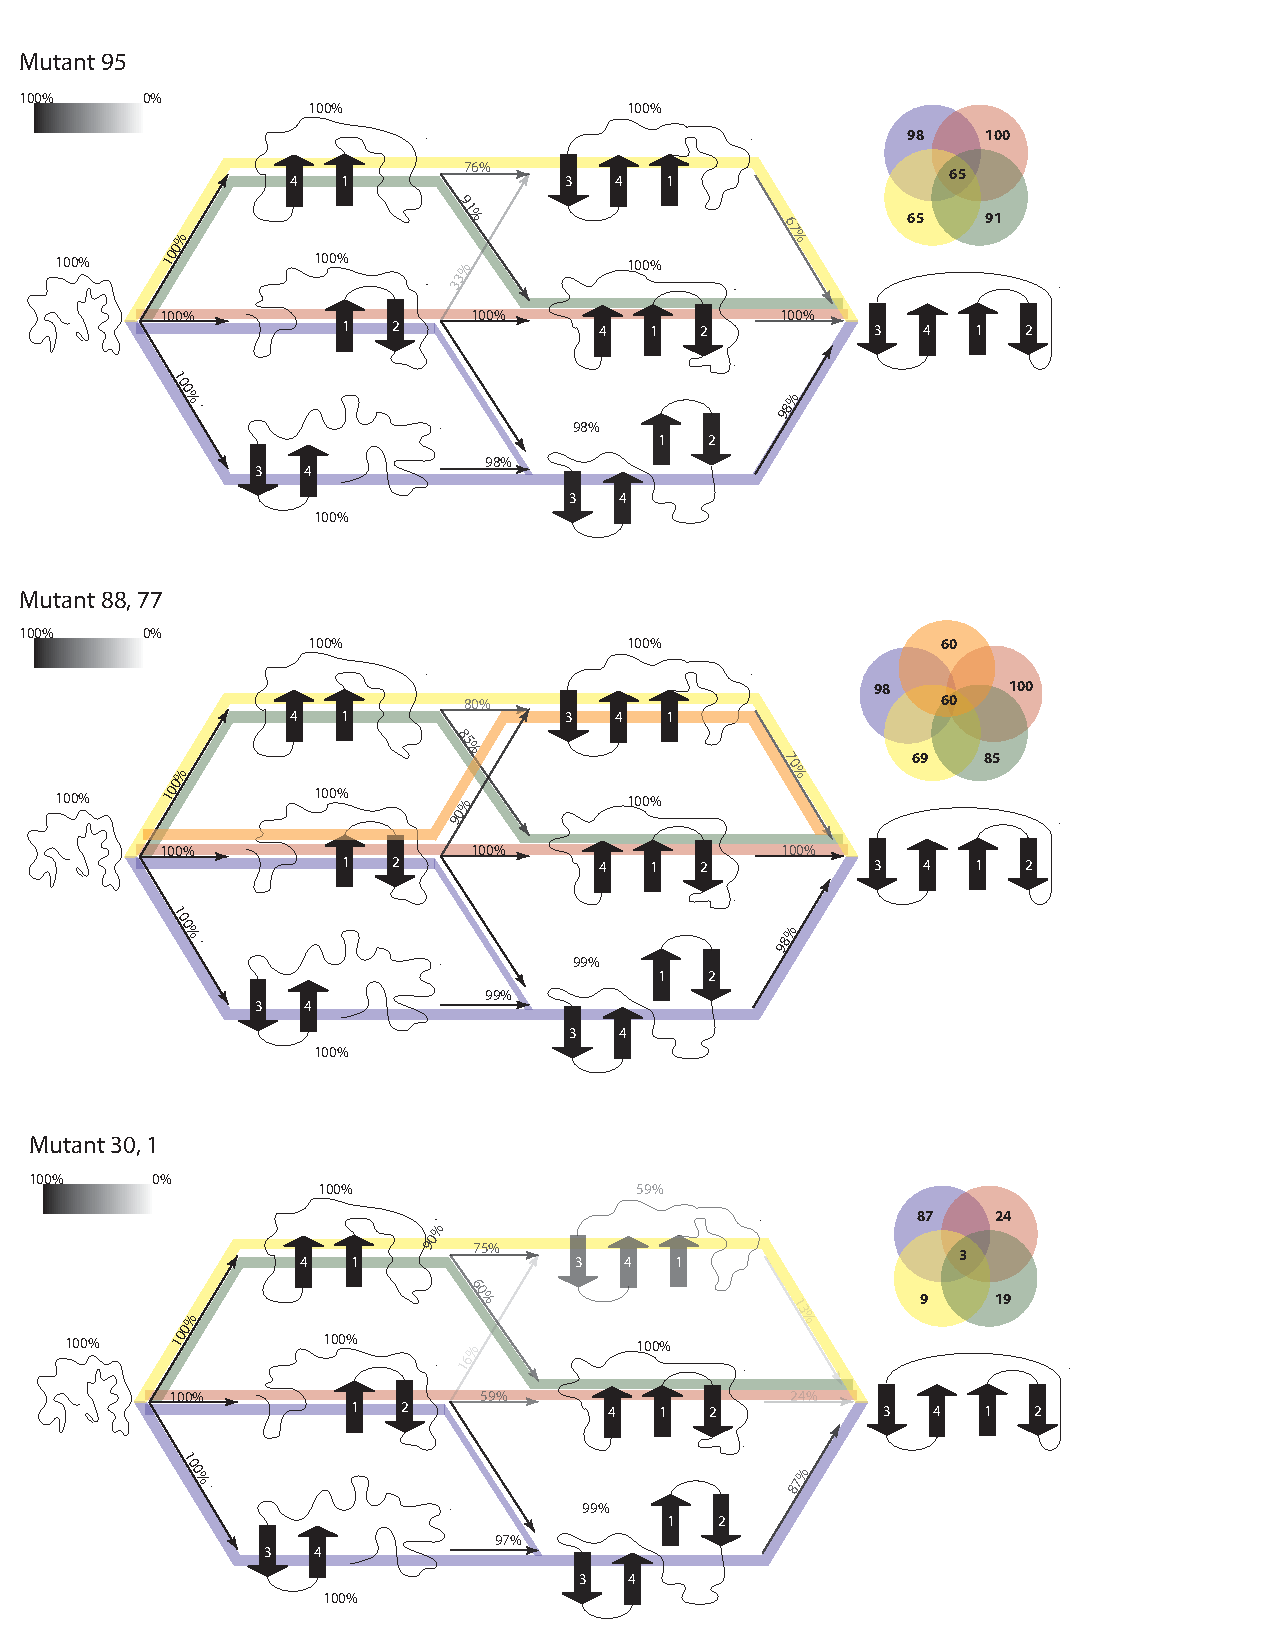
\includegraphics[scale=0.9, angle =0, clip=true, trim= 10 0 100 40]{Figures/Pathways_1EM7A.pdf}
			\caption{Pathways 1EM7A}  
		\label{fig:Pathways_1EM7A}
\end{figure*}

\begin{figure*}[htbp]
	 \centering
	 		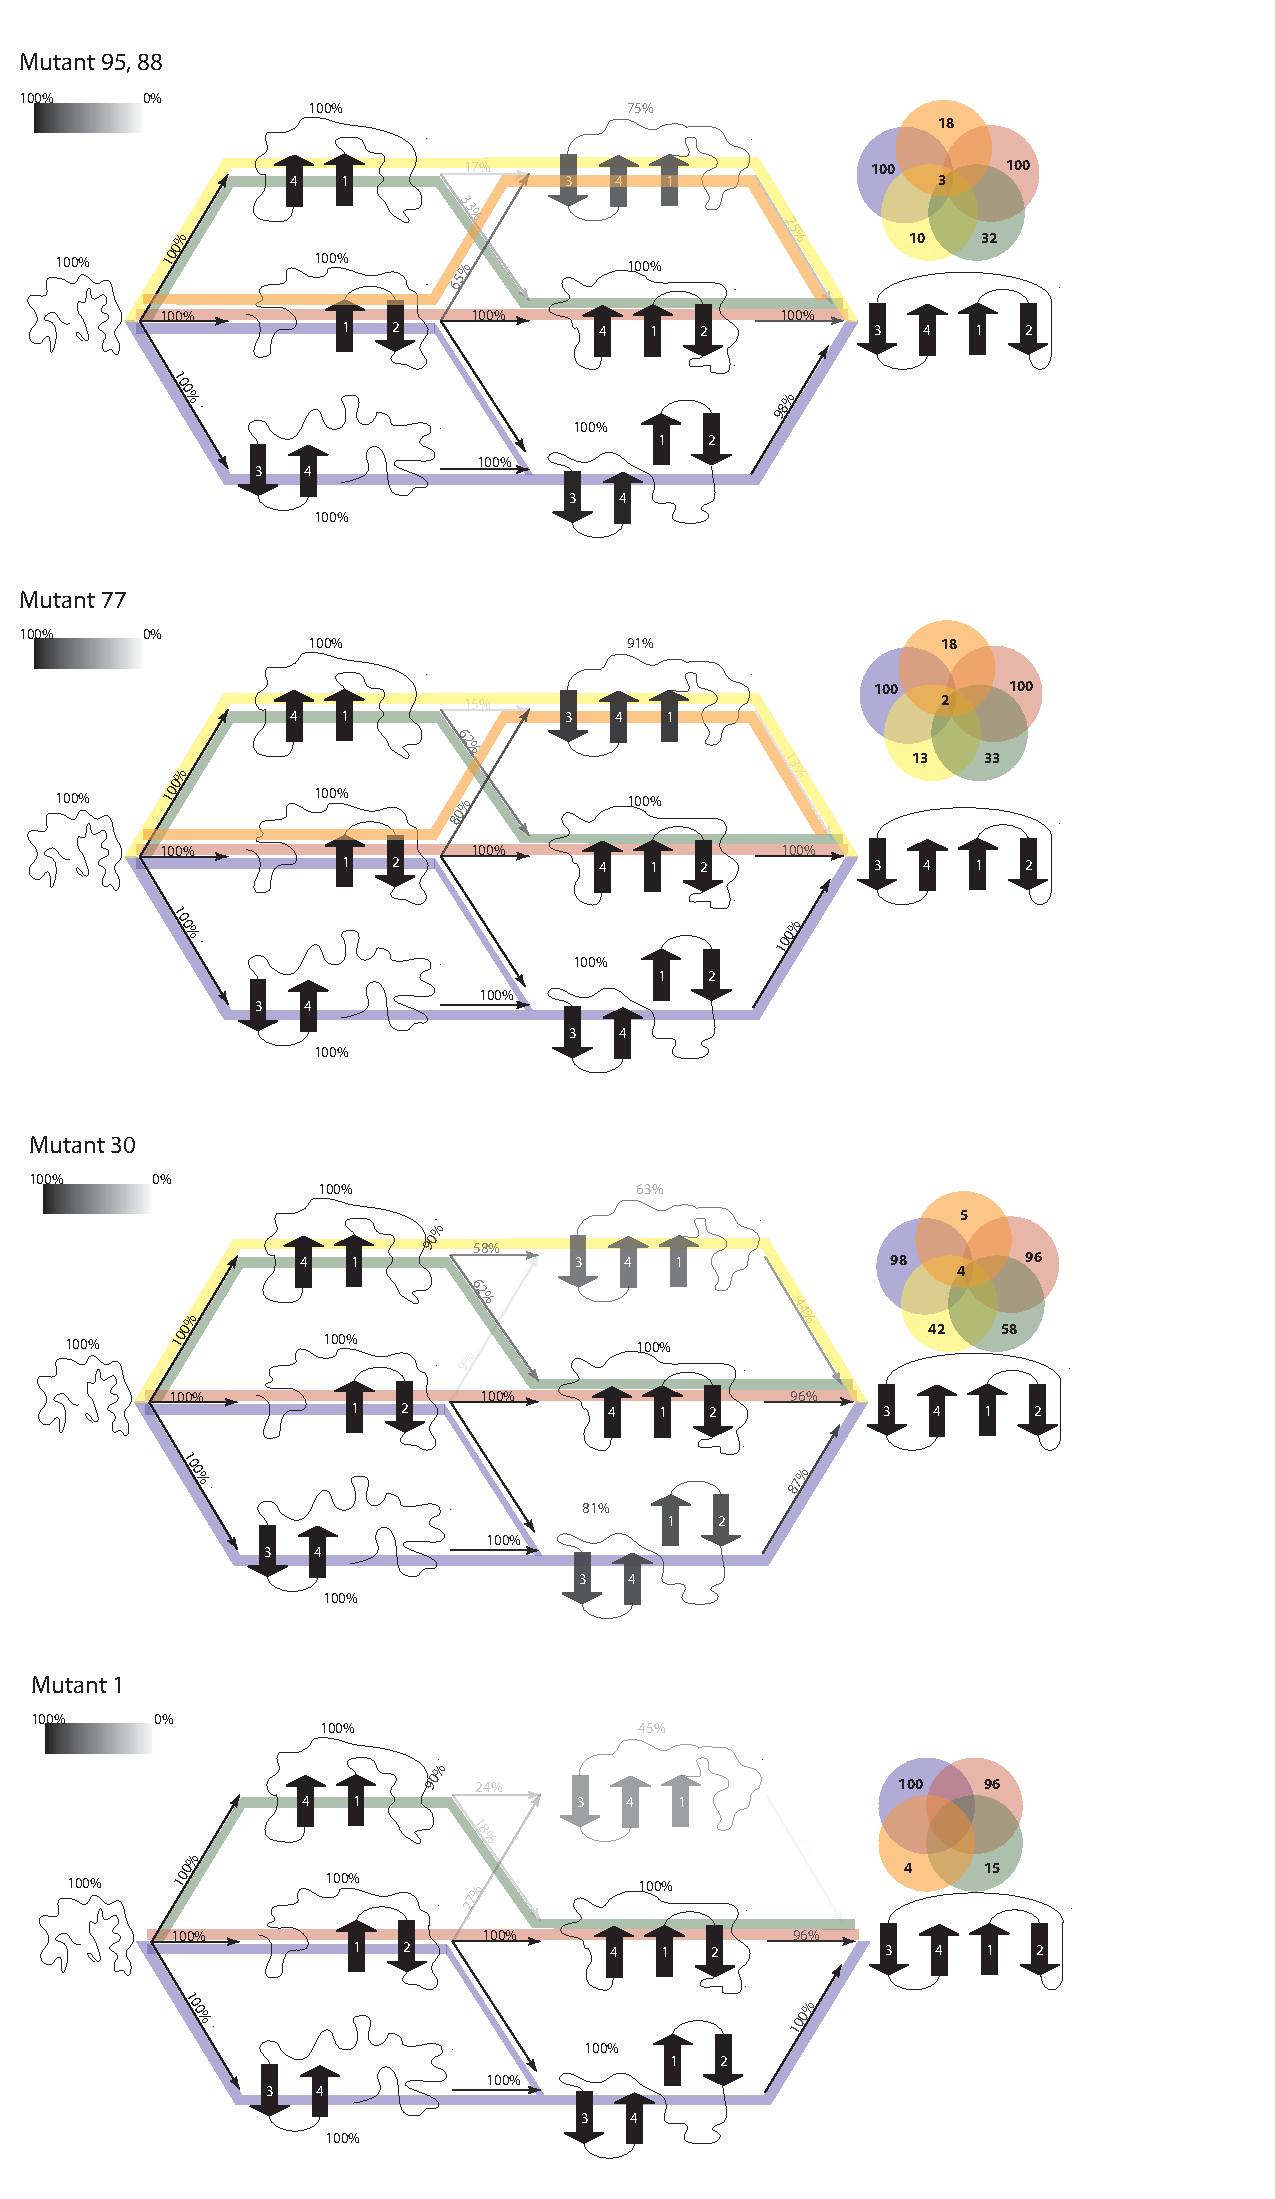
\includegraphics[scale=0.7, angle =0, clip=true,  trim= 10 0 100 40]{Figures/Pathways_1EM7B.pdf}
			\caption{Pathways 1EM7B}  
		\label{fig:Pathways_1EM7B}
\end{figure*}



\begin{tabular}{l| l*{10}{l}}
Protein & 1EM7 & B95 & A95 & B88 & A88  & B77 & A77 & B30 & A30 & B1 & A1 \\
\hline
1EM7 & 100 & 63 & 58 & 65 & 54 & 72 & 50 & 83 & 17 & 88 & 13 \\
B95 &  & 100 & 95 & 93 & 92 & 90 & 88 & 74 & 54 & 67 & 45  \\
A95 &  &  & 100 & 92 & 97 & 84 & 93 & 68 & 59 & 61 & 50  \\
B88 & &  &  & 100 & 88 & 93 & 84 & 77 & 50 & 70 & 42  \\
A88 &  &  &  &  & 100 & 81 & 97 & 65 & 63 & 58 & 54 \\
B77 &  &  &  &  &  & 100 & 77 & 84 & 43 & 77 & 34  \\
A77 &  &  &  &  &  &  & 100 & 61 & 67 & 54 & 58  \\
B30 &  &  &  &  &  &  &  & 100 & 31 & 93 & 24  \\
A30 &  &  &  &  &  &  &  &  & 100 & 24 & 92  \\
B1 &  &  &  &  &  &  &  &  &  & 100 & 17  \\
A1 &  &  &  &  &  &  &  &  &  &  & 100  \\
\end{tabular}



\begin{figure*}[htbp]
	 \centering
	 		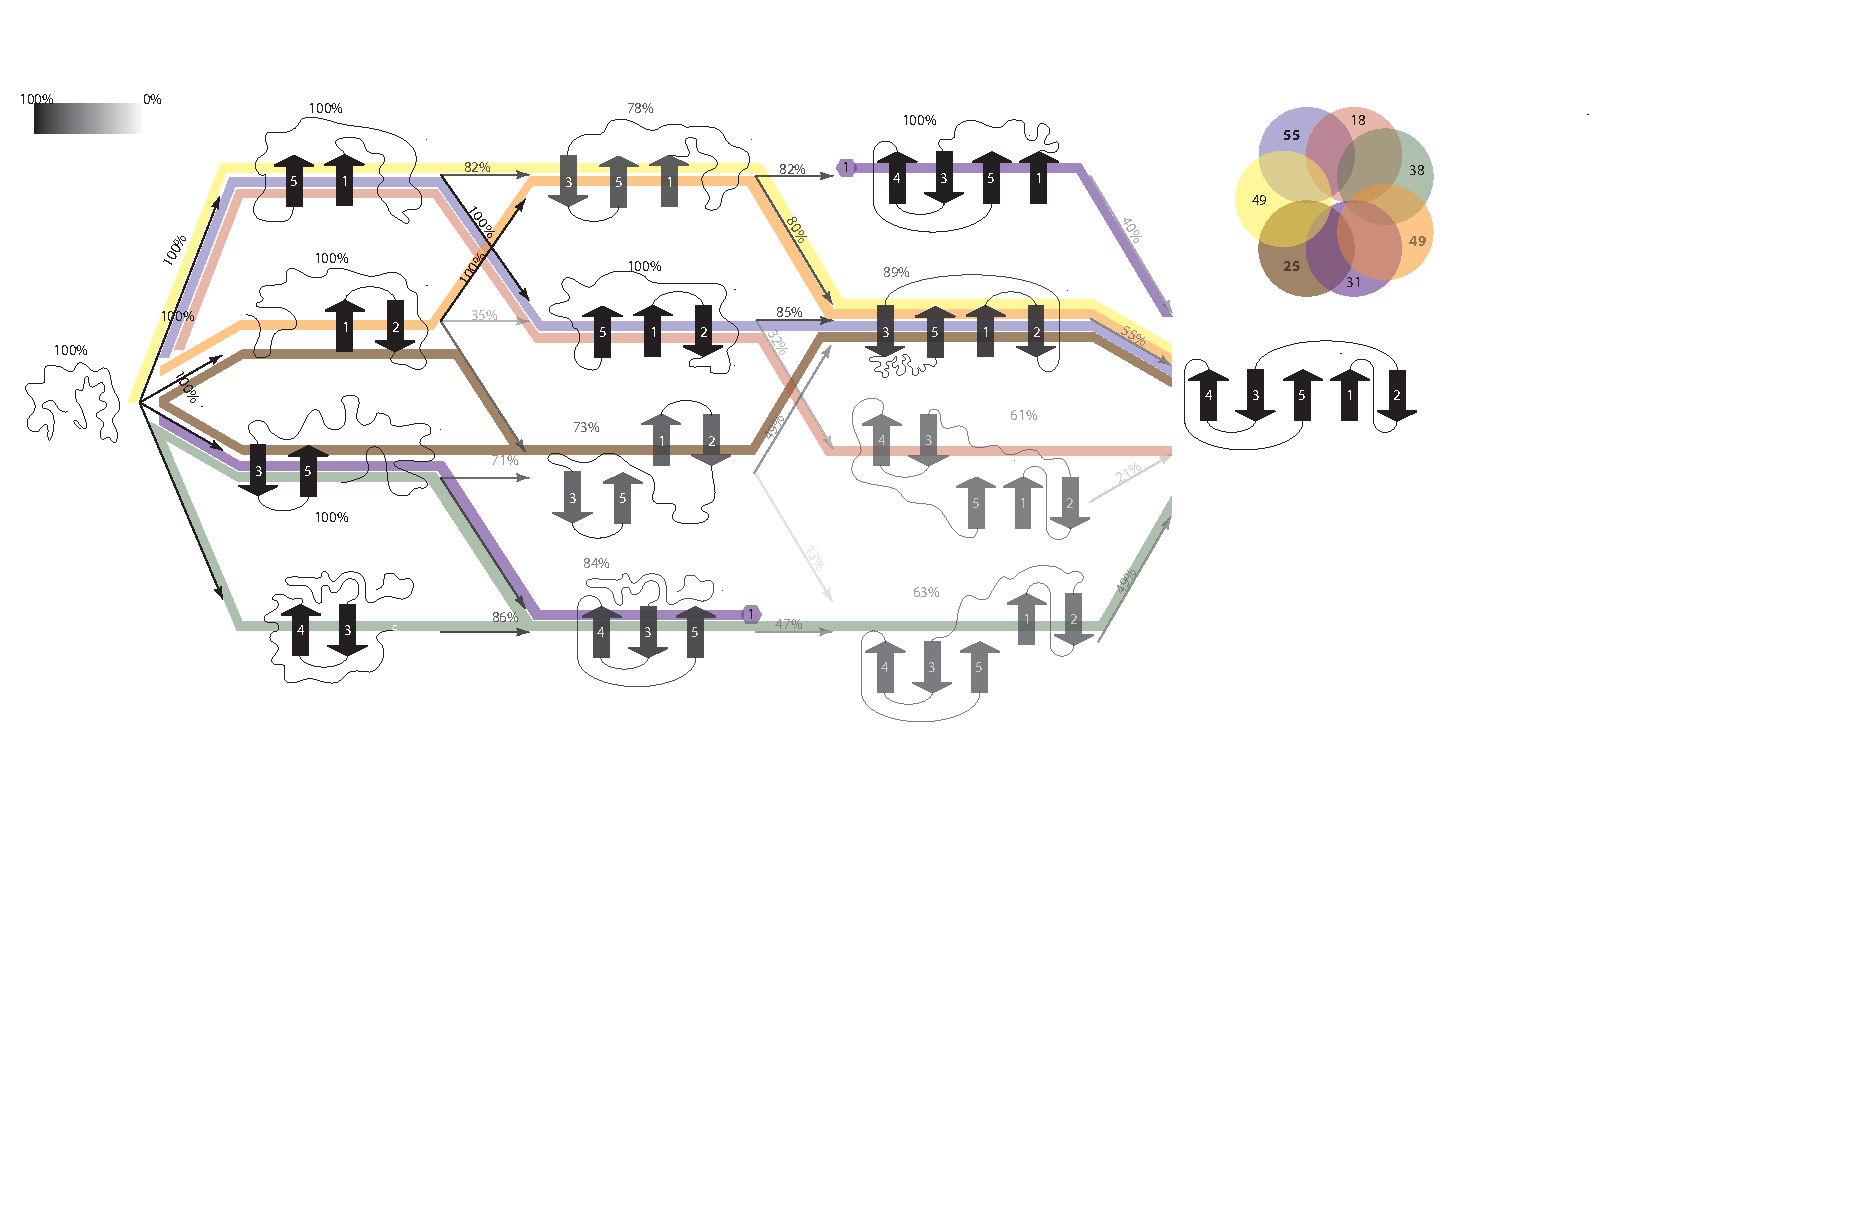
\includegraphics[scale=0.8, angle =0, clip=true, trim= 10 250 0 40]{Figures/Pathways_1UBQ.pdf}
			\caption{Pathways 1UBQ}  
		\label{fig:Pathways_1UBQ}
\end{figure*}

\begin{figure*}[htbp]
	 \centering
	 		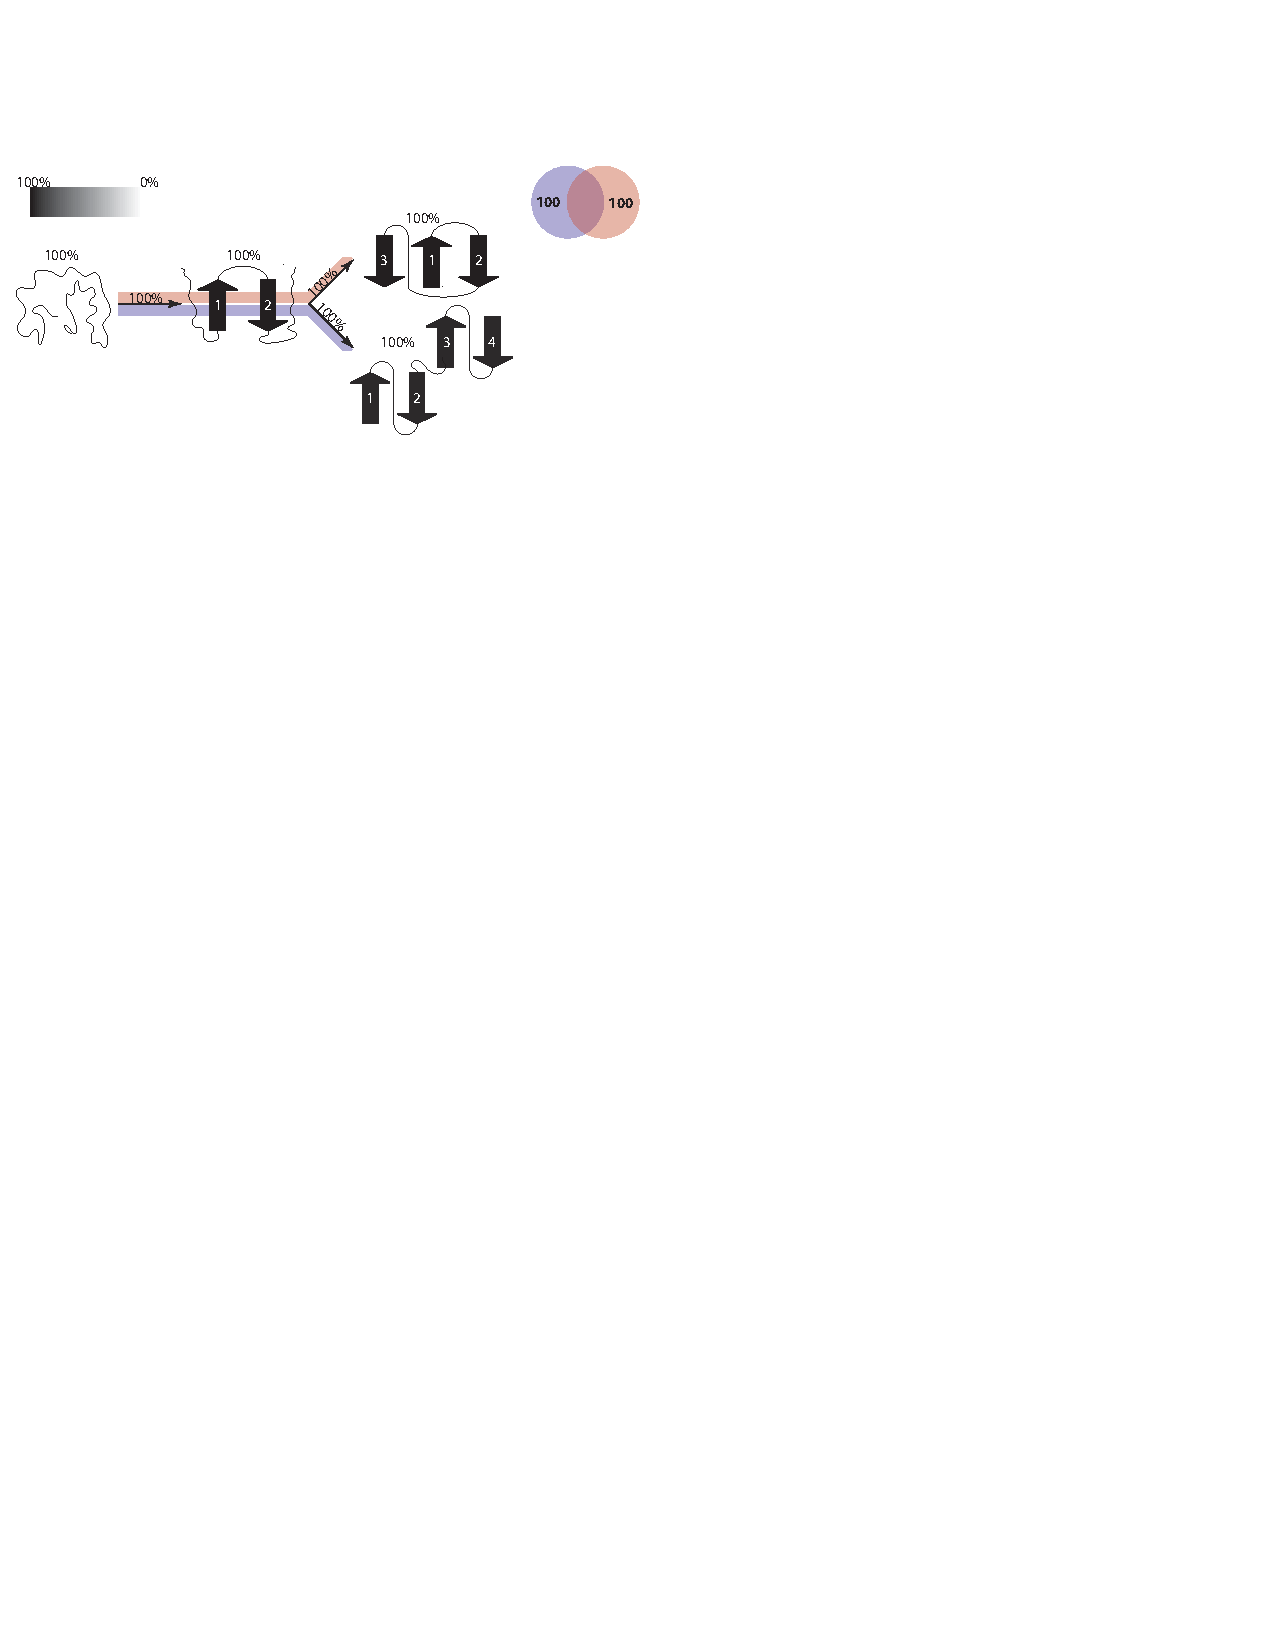
\includegraphics[scale=0.9, angle =0, clip=true, trim= 5 575 300 40]{Figures/Pathways_PF00014.pdf}
			\caption{Pathways PF00014}  
		\label{fig:Pathways_PF00014}
\end{figure*}

\begin{figure*}[htbp]
	 \centering
	 		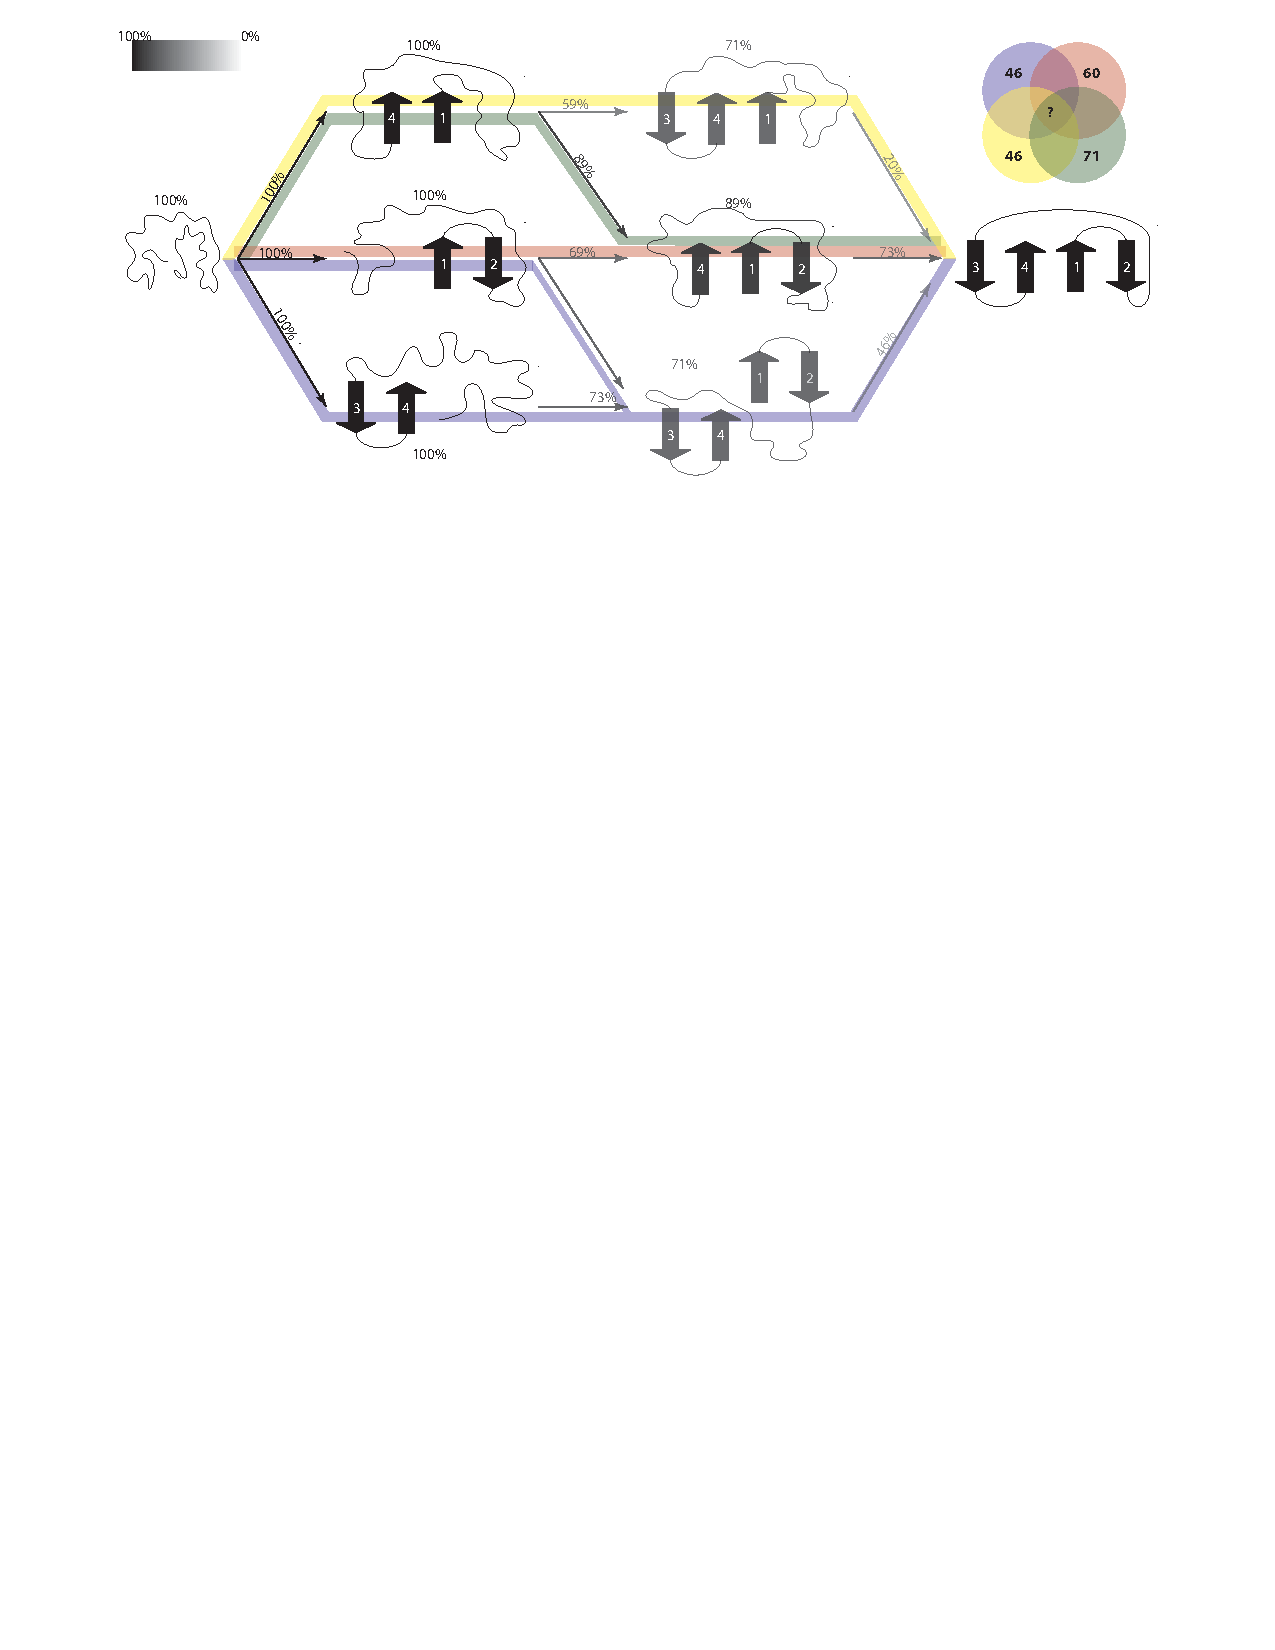
\includegraphics[scale=0.9, angle =0, clip=true,  trim= 10 550 50 10]{Figures/Pathways_PF00240.pdf}
			\caption{Pathways PF00240}  
		\label{fig:Pathways_PF00240}
\end{figure*}

\begin{figure*}[htbp]
	 \centering
	 		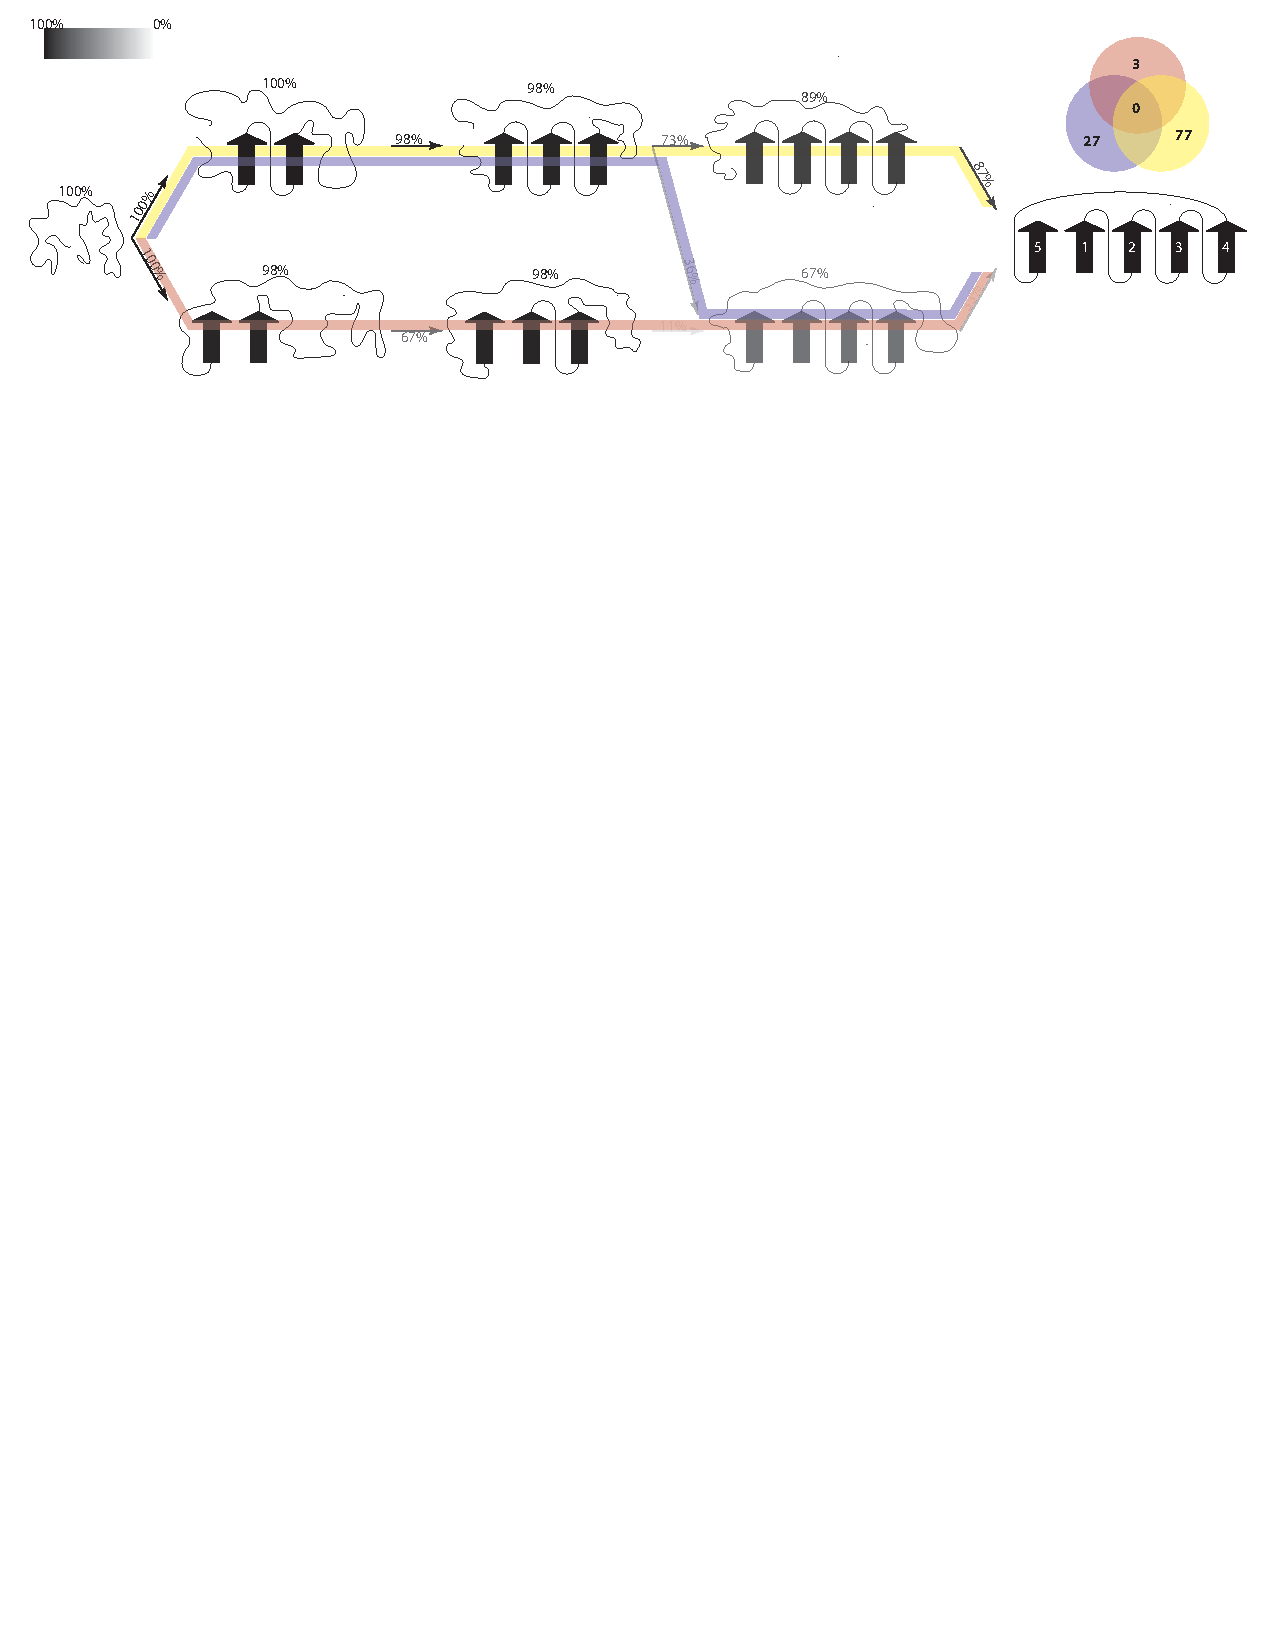
\includegraphics[scale=0.9, angle =0, clip=true, trim= 10 595 10 10]{Figures/Pathways_PF01423.pdf}
			\caption{Pathways PF01423}  
		\label{fig:Pathways_PF01423}
\end{figure*}

\begin{figure*}[htbp]
	 \centering
	 		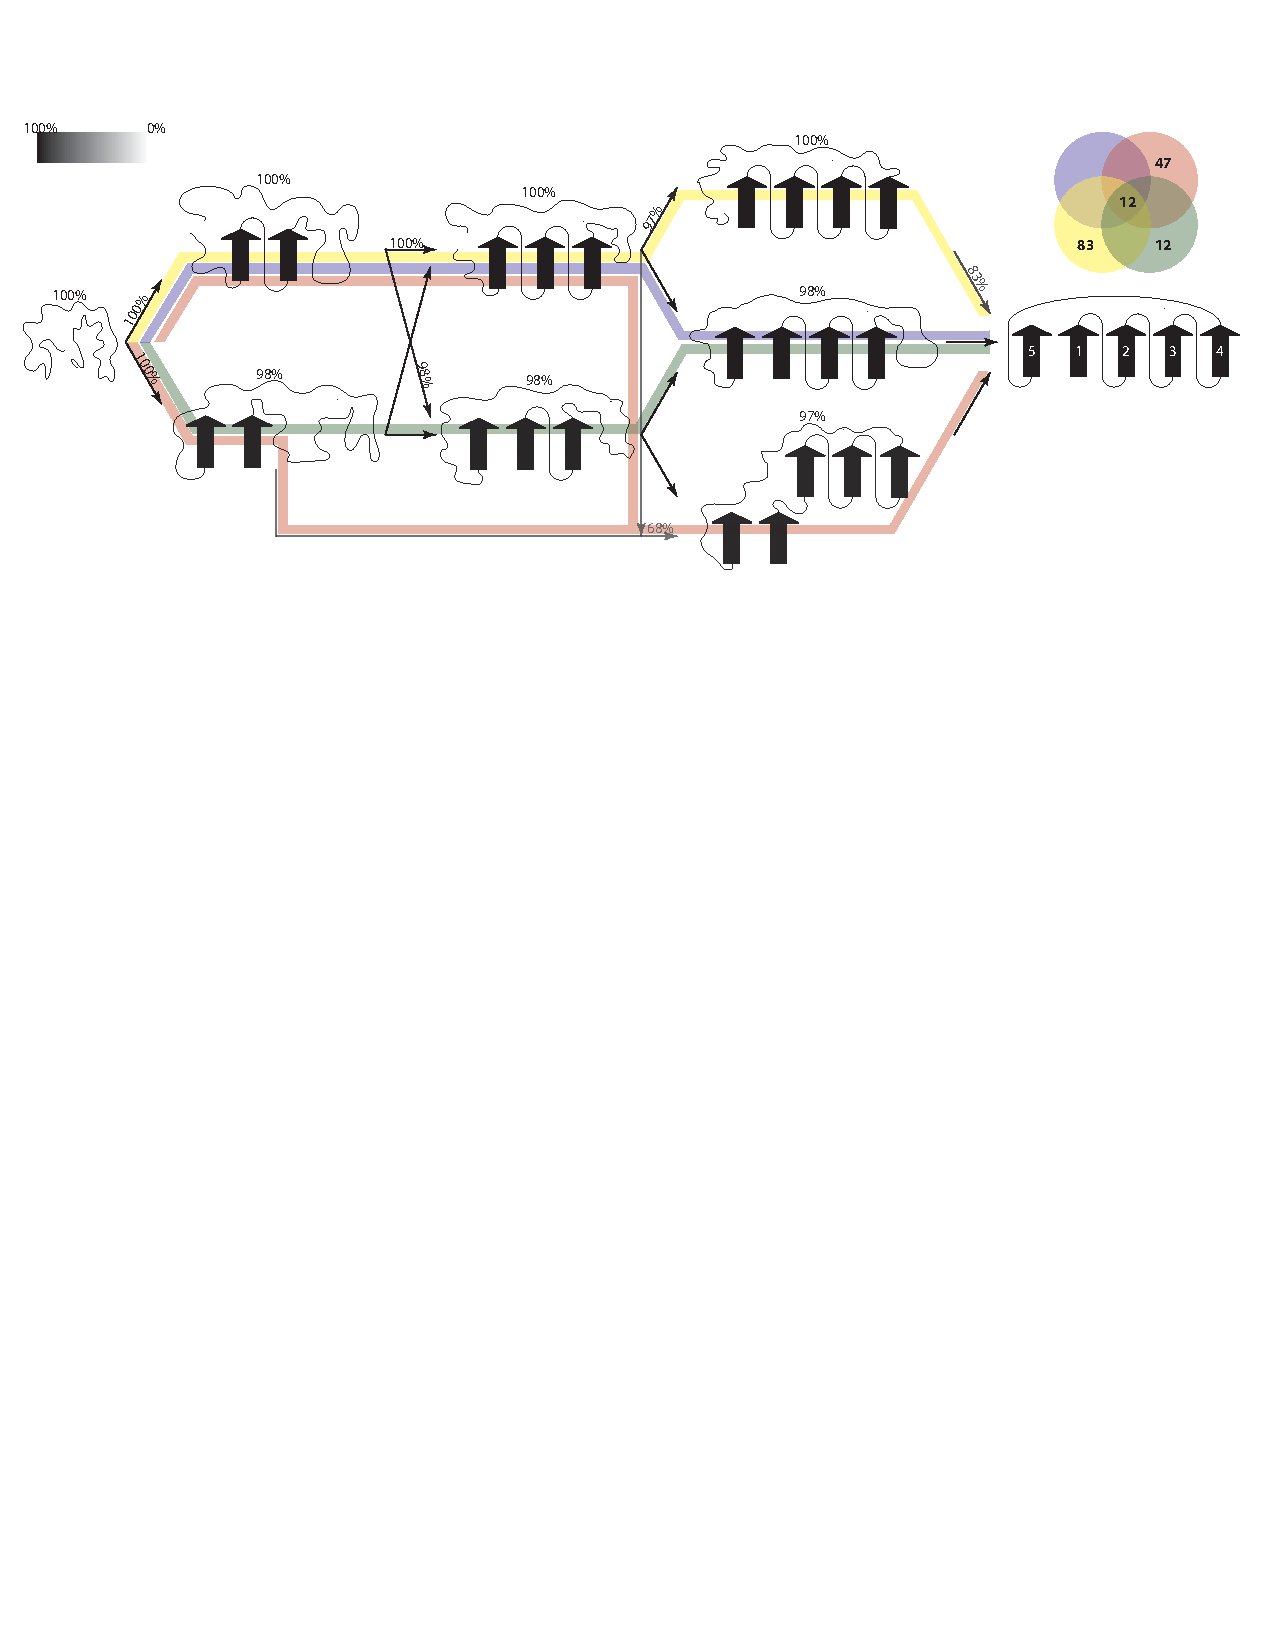
\includegraphics[scale=0.8, angle =0, clip=true, trim= 10 525 10 40]{Figures/Pathways_SH3.pdf}
			\caption{Pathways SH3}  
		\label{fig:Pathways_SH3}
\end{figure*}









\section{Conclusions}


\section{Report December 3, 2014}

\subsection{Conclusions of the experimental framework}




\begin{enumerate}
\item The proposed method improves the prediction of residue contacts.
\begin{itemize}
\item :) The proposed method improves the prediction of residue contacts with respect to our previous approach (compared with protein G).
\item :) The proposed method improves the prediction of $L_{500}$ for EvFold.
\item :) The proposed method predicts  residue contacts with an average greater that $50\%$ for all quality measures for $\pm2$ for all contact separations in the complete benchmark.. 
\item :) Exact prediction tends to be higher than $0.2$ for all the contact separations.
\item :) The precision of strand prediction is high in the benchmark. Specially for $\pm2$.
\item :) An ``homogeneous'' behaviour can be noted in the data set regardless the diversity of the benchmark. Furthermore, there is a good balance between contact and strand prediction. 
\item :| Our method is not a contact or secondary structure prediction method. However, our method is flexible enough to study TSs and nuclei  residues in different proteins. 
\item :( The variance for our results is very high, it can be explained given the diversity of our study 
\end{itemize}


\item The proposed method improves the prediction of protein topologies.
\begin{itemize}
\item :) The proposed method does not have the constrains imposed to our previous approach.
\item :) In average, the proposed approach ranks the target cluster in the top $2\%$. 
\item :| It is hard to correlate the rank results with folding dynamic results, however, we have the data and we can select some proteins to do that. 
\item :( The method predicts a lot of topologies. This prediction grows exponentially with the number of strands. It will be important to generate a filter during the running time.
\end{itemize}

\item The proposed method has a good prediction of protein pathways.
\begin{itemize}
\item :) The proposed method correlates well the in-silico data vs experimental data (3 full experiments). However this correlation is constrained by the level of detail given by our method and the lack of an helix analysis. Inspection of the results reveals that the folding intermediates are consisted with previous literature reports. Specifically, it is consistent with the work reported by (\cite{blanco1994short,kuszewski2008fast}), with respect to the early formation of the second hairpin ($\beta3 - ~turn -\beta4$) and its fundamental role in the folding process. Additionally, this second hairpin centers around known nucleation points W43, Y50, F54 that are strongly stabilized by three hydrophobic residues W43, Y45 , F52 (\cite{hubner2004commitment}). Our results also show the nucleation of the $\beta$-sheet residues between $\beta1$ and $\beta4$ as a next folding event (See permutation $3 ~ 4 ~1 ~2$ with pairings  $\mathit{ANTI ~NONE ~ANTI}$). This folding event can be preceded by the folding interaction between the $\alpha$-helix and the second hairpin as also reported in (\cite{kmiecik2008folding,song2002path}).  Interestingly, there are many interactions of three pairings (i.e., four $\beta$-strands), which agrees with previous findings about that four stranded $\beta$-sheets constitutes a metastable folding intermediate (\cite{neudecker2012structure}). This fact is very important because it gives a possible explanation about how the exposition of strand $\beta1$ and the four $\beta$-strand complex can lead the amyloid aggregation process.
\item :) The method is flexible enough to agree with different experimental results, even if those experiments are sometimes contradictory.
\item :| The method validate some reported experiments and explore some pathways do not reported, however, the method can not make any consistent claim about new biological discoveries.  
\item :| The method is  consistent in the prediction of TS. We were able also to study nuclei residues.
\item :( First folding options do not agree with reported pathways.
\end{itemize}

\item The proposed method is able to discriminate and differentiate protein pathways even in high similar protein sequences.
\begin{itemize}
\item :) The rank for proteins belonging to the ``B" mutant group is better than the its ``A" counterpart.
\item :) The pathways of the ``B" mutant group keeps similarities with the ``wildtype" group, however, there are also differences.
\item :) There are examples of similar sequences can keep very different pathways, also there are examples of similar sequences with similar pathways.
\item :) There are many combination to get conclusions.
\item :) The TS and nuclei residues are conserved. The bad news is that they are also conserved for the mutant A.
\item :( We do not have experimental data for the mutants.
\item :( We do not have a way to model the helices. 
\end{itemize}

\item The proposed method is able to identify recurrent states of proteins belonging to a same PFAM family.
\begin{itemize}
\item :) Pathways make sense with the structural features of the family.
\item :) Family PF00240 contains 1UBQ and family  PF00018 contains SH3. 
\item :| Problems validating the recurrent states. The folding pathways of disulphide proteins (Familly PF00014) vary substantially (BPTI vs TAP). Our study is based on BPTI and AMBP, there is no information about them.
\end{itemize}

\item The proposed method is able to identify recurrent states of proteins belonging to different PFAM families.
\begin{itemize}
\item :) We were able to compare the nucleus residues of proteinG with ubiquitin family. 
\item :) We were able to compare the pathways of proteinG with the ubiquitin family. 
\item :| Our study is based on the PFAM paradigm, what about other organization models? SCOP to name one?.
\end{itemize} 

\end{enumerate}

TO DO LIST....................

\begin{enumerate}
\item Write down a paragraph for each of the conclusions listed previously.
\item Write down the conclusions.
\item Write down the abstract.
\item Filter the sections and paragraphs in the paper.
\item Choose a journal.
\item Write down the editor letter.
\item To clean the code.
\item To set the web service.
\end{enumerate}



 















\bibliographystyle{unsrt}
\bibliography{eFold}

\end{document}